\documentclass{article}
\usepackage{graphicx}
\usepackage{amsmath}
\usepackage{amsfonts}
\usepackage{amssymb}
\usepackage{stmaryrd}
\usepackage{makeidx}
\usepackage{times}
\usepackage{mathptmx}
%Uncomment next line for pdflatex and use includegraphics with eps file
% for latex2html don't use the option [width=\textwidth]
% check that xfig files are exported magnif 100%
\usepackage{ifpdf}
\ifpdf
 \usepackage[colorlinks,pdftex]{hyperref}
\else
%\usepackage[ps2pdf,breaklinks=true,colorlinks=true,linkcolor=red,citecolor=green]{hyperref}
\fi
%\usepackage[francais]{babel}
\usepackage[T1]{fontenc}
%\DeclareGraphicsExtensions{.pdf, .png, .mps, .eps}
\newcommand{\R}{{\mathbb{R}}}
\newcommand{\C}{{\mathbb{C}}}
\newcommand{\Z}{{\mathbb{Z}}}
\newcommand{\N}{{\mathbb{N}}}
\newcommand{\faux}{$\square\;$}
\newcommand{\vrai}{$\boxtimes\;$}
\newcommand{\itemf}{\item\faux}
\newcommand{\itemvv}{\item\vrai}
\newcommand{\xcasin}[1]
{\begin{quote}\ttfamily
#1
\end{quote}}
\newcommand{\xcasout}[1]
{\begin{equation*}
#1
\end{equation*}}

%---------------------------------------------
\newtheorem{exo}{Exercise}[section]
\makeindex
%---------------------------------------------
\begin{document}
\vspace*{1cm}
\begin{center}
{\Huge An \texttt{Xcas} Tutorial}
\end{center}

\tableofcontents

\newpage

\texttt{Xcas} is a free (as in Free Software) computer algebra system.
Although there are other computer algebra systems, both free and
commercial, few if any are as versatile as \texttt{Xcas},
which is capable of, among other things:
\begin{itemize}
  \item
  Symbolic and numeric calculation.
  \item
  Programming.
  \item
  Graphing functions.
  \item
  Working with spreadsheets.
  \item
  Interactive geometry (both two- and three-dimensional).
  \item
  Turtle geometry.
\end{itemize}
This tutorial will briefly introduce a new user to calculating,
programming and graphing with \texttt{Xcas}.  The first section, 
``Getting started'', will be just enough information to get you
started.  The second section will be a brief overview of the
graphic interface and the rest will be more in-depth tutorial.

For more information, you can refer to the manual or any of the other
sources of information under the \texttt{Help} menu.

\section{Getting started}

\subsection{Starting \texttt{Xcas}}

\texttt{Xcas} is available from 
\url{http://www-fourier.ujf-grenoble.fr/~parisse/giac_fr.html}.
This page also has information on installation.  Once installed, the
way to start the program depends on the operating system.
\begin{itemize}
  \item
  Under Windows, there should be a shortcut \texttt{xcasen.bat} that
  you can click on.
  \item
  Under Linux, you can either find it on a menu provided by the
  desktop environment, or enter \texttt{xcas \&} in a terminal window.
  \item
  Under MacOS, you can click on \texttt{xcas} in the Applications menu.
\end{itemize}
For this tutorial, you will mostly be working with the
command line, which will be a white rectangle next to the number
\texttt{1}.  There you can enter a command, after which there will be
a window with the result, followed by another command line with the
number \texttt{2}.

\subsection{\texttt{XCas} as a calculator}

Once you have started \texttt{Xcas}, you can immediately use it as a
calculator.  Simply type in the expression that you wish to
use, using the standard arithmetic operators; namely \texttt{+} for
addition, \texttt{-} for subtraction, \texttt{*} for multiplication,
\texttt{/} for division and \texttt{\^{}} for exponentiation.
If you enter
\xcasin{34+45*12}
you will get
\xcasout{574}
If you enter
\xcasin{2/3 + 98/7}
you will get
\xcasout{\frac{44}{3}}
The operators have a standard order of operations, and parentheses
can be used for grouping.  (Brackets have a different meaning, see
section \ref{lists}, ``Lists, sequences and sets''.)

Notice that if you enter integers or other exact values,
\texttt{Xcas} will give you the exact result.  If you enter an
approximate value, such as a number with a decimal point (computers
regard numbers with decimal points as approximate values), then
\texttt{Xcas} will give you an approximate result.  For example, if
you enter
\xcasin{2/3 + 3/2}
you will get
\xcasout{\frac{13}{6}}
but if you enter
\xcasin{2/3 + 1.5}
you will get
\xcasout{2.16666666667}
You can also get a decimal approximation using the \texttt{evalf}
function.  If you enter
\xcasin{evalf(2/3 + 3/2)}
you will get
\xcasout{2.16666666667}
By default, \texttt{Xcas} will give you 12 decimal places of accuracy
in its approximations, but this is configurable (see section
\ref{config}, ``Configuration'').

\texttt{Xcas} also has the standard functions, such as
\texttt{sin}, \texttt{cos}, \texttt{asin} (for the arcsin),
\texttt{log} (for the natural logarithm).
It also has common constants such as \texttt{pi}, \texttt{e} and \texttt{i}.

The trigonometric functions assume that angles are measured in
radians.  (This can be configured, see section \ref{config},
``Configuration''.)  If you enter
\xcasin{sin(pi/4)}
you will get
\xcasout{\frac{\sqrt{2}}{2}}

\subsection{Functions and variables}

\texttt{Xcas} can work with expressions and variables as well as numbers.
A variable in \texttt{Xcas} needs to begin with a letter and can
include numbers and underscores. If you enter
\xcasin{x\^{}2 + x + 2*x + 2}
you will get
\xcasout{x^2 + 3*x + 2}
You can give a variable a value with the assignment operator,
\texttt{:=}.  To assign the variable \texttt{myvar} the value 5, for
example, you could enter
\xcasin{myvar := 5}
If you used \texttt{myvar} in an expression, it would then be replaced
by \texttt{5}; entering
\xcasin{myvar*x + myvar\^{}2}
would result in
\xcasout{5*x + 25}

The assignment operator can also be used to define functions.  To
define the squaring function, for example, you could enter
\xcasin{sqr(x) := x\^{}2}
Afterwards, whenever you enter \texttt{sqr(expression)} you will
get the expression squared.  For example, entering
\xcasin{sqr(7)}
would return
\xcasout{49}
and entering
\xcasin{sqr(x+1)}
would result in
\xcasout{(x+1)^2}

\subsection{Simplifying expressions}

When you enter an expression into \texttt{Xcas}, some simplifications
will be done automatically.  For example, if you enter
\xcasin{a := 3}
\xcasin{b := 4}
and
\xcasin{a*b*x + 4*b\^{}2}
you will get
\xcasout{12*x + 64}

\texttt{Xcas} has several transformations in case you want an
expression to be simplified beyond the automatic simplifications, or
perhaps transformed in another way.  Some examples are:
\begin{description}
  \item[\texttt{expand}]
  This will expand integer powers, and more generally distribute
  multiplication across addition.  For example, if you enter
  \xcasin{expand((x+1)\^{}3)}
  you will get
  \xcasout{x^3 + 3*x^2 + 3*x + 1}
  
  \item[\texttt{factor}]
  This will factor polynomials.  For example, if you enter
  \xcasin{factor(x\^{}2 + 3*x + 2)}
  you will get
  \xcasout{(x + 1)*(x + 2)}
\end{description}  

\subsection{Graphs}

\texttt{Xcas} has several functions for plotting graphs; perhaps the
simplest is the \texttt{plot} function.  The \texttt{plot} function
requires two arguments, an expression to be graphed and a variable.
For example, if you enter
\xcasin{plot(sin(x),x)}
you will get the graph
\begin{center}
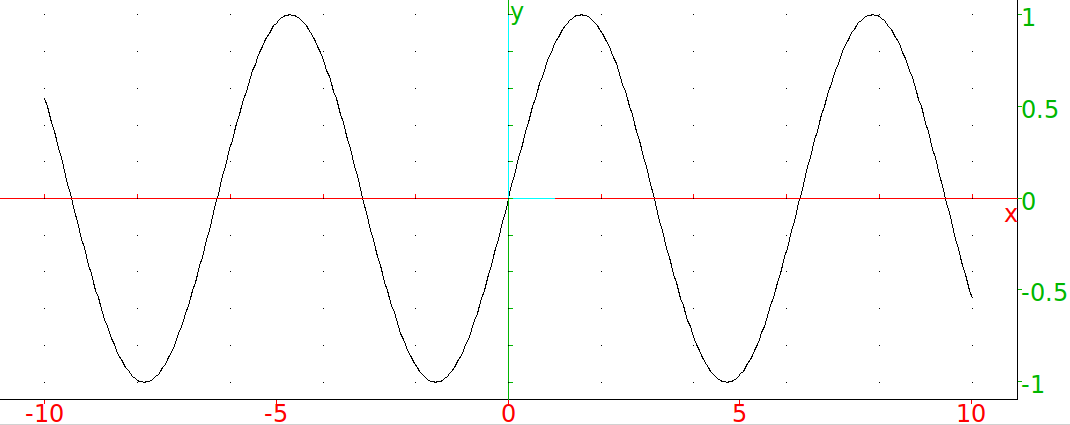
\includegraphics[width=\textwidth]{xcas-sinplot.png}
\end{center}
To the right of the graph will be a panel you can use to control
various aspects.  By default, the graph will cover values of the
variable from $-10$ to $10$; this is of course configurable (see
section \ref{config}, ``Configuration'').  To plot
over a different interval, you can also use a second argument of 
\textit{var}=\textit{min}..\textit{max} instead of simply
\textit{var}.  For example, if you enter
\xcasin{plot(sin(x),x=-pi..pi)}
you will get the graph
\begin{center}
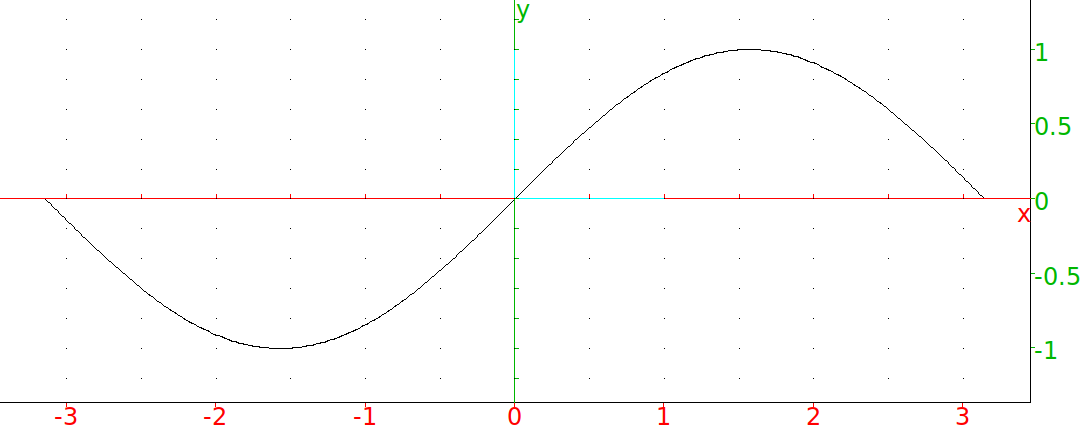
\includegraphics[width=\textwidth]{xcas-sinplot2.png}
\end{center}

\subsection{The Help Index}

You can get a list of all \texttt{Xcas} commands and variables using the
\texttt{Help$\blacktriangleright$Index} menu item.  This will bring up
the following window:
\begin{center}
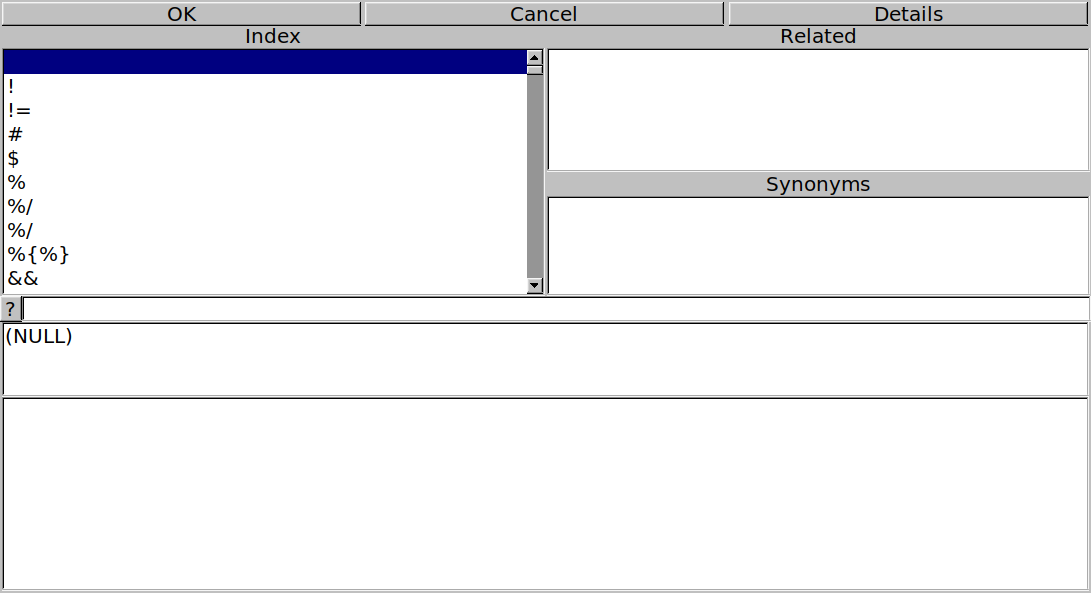
\includegraphics[width=\textwidth]{xcas-help-index.png}
\end{center}
Under \texttt{Index} will be a scrollable list of all the commands and
variables.  
If you begin typing to the right of the question mark, you will be
taken to the part of the list beginning with the characters you typed;
for example, if you type \texttt{evalf}, you will get the following:
\begin{center}
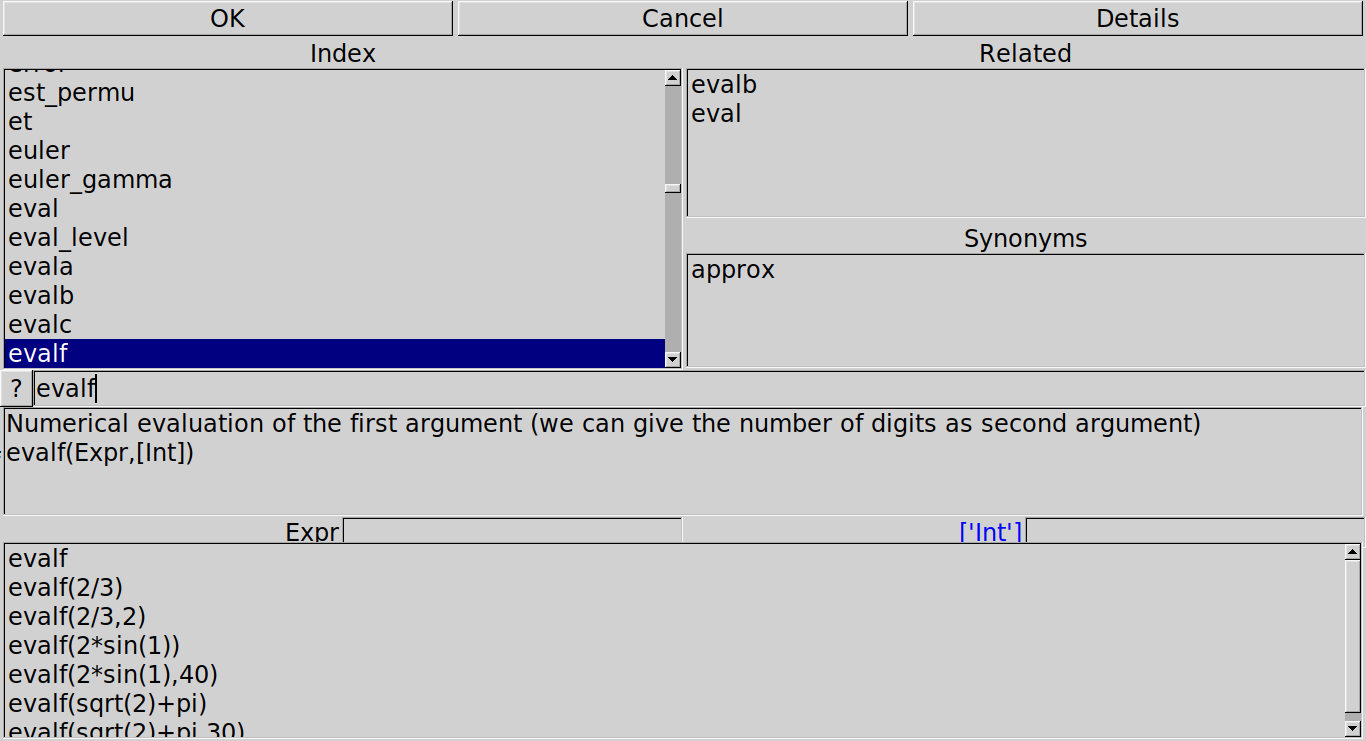
\includegraphics[width=\textwidth]{xcas-help-evalf.png}
\end{center}
In the upper right-hand pane under \texttt{Related} is a list of
commands related to the chosen command, below that is a list of
synonyms; you can see that the \texttt{approx} command is the same as
the \texttt{evalf} command.  Below the line where you typed the
command you are looking up is a description of the command; here you
can see that \texttt{evalf} takes an optional second argument
(brackets in the description indicate that an argument is optional)
which can specify the number of digits in the approximation; for
example, 
\xcasin{evalf(pi)}
will return
\xcasout{3.14159265359}
but 
\xcasin{evalf(pi,20)}
will return
\xcasout{3.1415926535897932385}
Below the description is a line where you can enter the arguments for
the command; if you enter values in these boxes then the command with
the chosen arguments will be placed on the \texttt{Xcas} command line.
At the bottom of the help window is a list of examples of the command
being used; if you click on one of these examples it will appear on
the \texttt{Xcas} command line.

As well as using the menu, you can get to the help index by using the
tab key while at the \texttt{Xcas} command line.  If you have typed
the beginning of a command before using the tab key, then that
beginning will be presented to you in the help index.

\section{The interface}

\subsection{Overview}

When you start \texttt{Xcas}, you will be presented with a window which
looks like the following:
\begin{center}
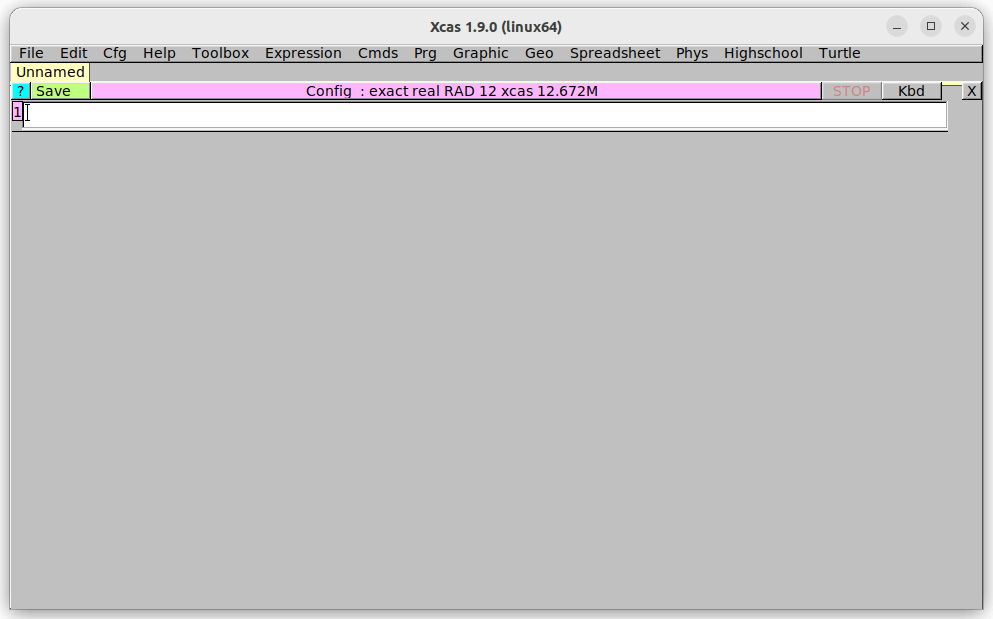
\includegraphics[width=\textwidth]{xcas-open.png}
\end{center}
From top to bottom, there is
\begin{itemize}
  \item
  A menu bar.
  \item
  A tab indicating the name of the session, or \texttt{Unnamed} if the
  session has not been saved.  You can run several sessions
  simultaneously, in which case each session will get its own tab.
  \item
  A session management bar, with
  \begin{itemize}
    \item
    A \texttt{?} button, which will open the help index.
    \item
    A \texttt{save} button to save the session.
    \item
    A configuration button, indicating how \texttt{Xcas} is currently
    configured.  Clicking on this button will open a configuration
    window.
    \item
    A \texttt{STOP} button you can use to interrupt a calculation
    which is running on too long.
    \item
    A \texttt{Kbd} button to bring up an on-screen keyboard which you
    can use to help enter your commands.  It will come with a control panel
    which you can use to display a message window (\texttt{msg}) or
    show an extra menu (\texttt{cmds}) at the bottom.
    \item
    An \texttt{X} button to close the session.
  \end{itemize}
  \item
  A numbered command line.
\end{itemize}

\subsection{The menu bar}

The menu items have submenus, and sometimes sub-submenus. When
indicating a submenu item, it will be separated from the menu item with
$\blacktriangleright$; for example, you can save a session with
\texttt{File$\blacktriangleright$Save}, which is the \texttt{Save}
item in the \texttt{File} menu.

The menu bar contains the usual menus for graphic programs.  It also
contains all of the \texttt{Xcas} commands grouped by themes.  For
some commands, if you choose it from a menu then the command will be
put on the command line.  If the message window is open (which you can
open with the
\texttt{Cfg$\blacktriangleright$Show$\blacktriangleright$msg}
menu item), a brief description of the command will appear in that
window.  For other commands, for example the \texttt{Graphic}
commands, you will get a dialog box which lets you specify the
arguments; afterwards, the command with the arguments will be placed
on the command line.

The \texttt{Help} menu has links to the Help index, various manuals,
as well as the online forum.  

\subsection{Configuration}
\label{config}

The \texttt{Cfg} menu has various items that allow you to configure
various aspects of \texttt{Xcas}.  This tutorial will
refer to the \texttt{Cfg$\blacktriangleright$Cas configuration} and 
\texttt{Cfg$\blacktriangleright$Graph configuration} menu items.  The
\texttt{Cfg$\blacktriangleright$Cas configuration} menu item will
bring up the same configuration page as clicking on the status bar.
These items will bring up windows with various entry fields and
check boxes; after you make any changes, you can click the
\texttt{Apply} button to apply them and the \texttt{Save} button to
save them for future sessions.

The \texttt{Cfg$\blacktriangleright$Cas configuration} menu item will
bring up a window with options that determine how \texttt{Xcas} computes.
This includes some things mentioned in this tutorial, such as:
\begin{itemize}
  \item
  \textbf{Digits.}
  This entry field determines the number of significant digits used in
  calculations.  This resets the value of the variable \texttt{Digits},
  which you can also reset from the command line.
  \item
  \textbf{epsilon.}
  This entry field determines how close the fraction returned by
  \texttt{exact} will be to the input.  This resets the value of the
  variable \texttt{epsilon}, which you can also reset from the command
  line.
  \item
  \textbf{radian.}
  This checkbox determines whether angles are measured in radians or
  degrees.
  \item
  \textbf{Complex.}
  This checkbox determines whether computations will find complex
  solutions to equations.
  \item
  \textbf{All\_trig\_sol.}
  This checkbox determines whether \texttt{solve} will find the
  primary solutions to trigonometric equations or all solutions.
\end{itemize}

The \texttt{Cfg$\blacktriangleright$Graph configuration} menu item
will bring up a window with options that determine how \texttt{Xcas}
draws graphs.  This includes the default ranges for the axes; the
$x$-axis will go from \texttt{X-} to \texttt{X+}, the $y$-axis will go
from \texttt{Y-} to \texttt{Y+} and the $z$-axis will go from
\texttt{Z-} to \texttt{Z+}.

\subsection{The command line}

You can run a command by typing it into the command
line and pressing \texttt{Enter}.  If you want to enter more than one
command on a line, you can separate them with semicolons.  If you want
to suppress the output of a command, you can end it with a
colon-semicolon (\texttt{:;}).

If you have enough commands, there will be a scroll bar on the right
which you can use to scroll through different command line levels.  The
\texttt{Edit} menu will allow you to merge levels, group levels and
add comments.

All commands are kept in memory.  You can scroll through previous
commands with \texttt{Ctrl+} arrow keys, and modify them if you want.

\section{Computational objects}

\subsection{Numbers}

\begin{center}
\begin{tabular}{|p{.20\textwidth}|p{.6\textwidth}|}
\hline
\multicolumn{2}{|c|}{\textbf{Operations}}\\
\hline\hline
\texttt{+}    & addition\\
\texttt{-}    & subtraction \\
\texttt{*}    & multiplication  \\
\texttt{/}    & division\\
\texttt{\^{}} & power  \\
\hline
\end{tabular}
\end{center}
\index{addition}
\index{subtraction}
\index{multiplication}
\index{division}
\index{power}

\begin{center}
\begin{tabular}{|p{.20\textwidth}|p{.6\textwidth}|}
\hline
\multicolumn{2}{|c|}{\textbf{Conversions}}\\
\hline\hline
\texttt{evalf}   & approximate a number\\
\texttt{exact}   & find an exact number close to the given number\\
\texttt{epsilon} & determine how close a fraction has to be to
                   a floating point number to be returned by
		   \texttt{exact}\\
\hline
\end{tabular}
\end{center}
\index{evalf@{\texttt{evalf}}}
\index{exact@{\texttt{exact}}}
\index{epsilon@{\texttt{epsilon}}}

\begin{center}
\begin{tabular}{|p{.20\textwidth}|p{.6\textwidth}|}
\hline
\multicolumn{2}{|c|}{\textbf{Constants}}\\
\hline\hline
\texttt{pi}  & $\pi\simeq 3.14159265359$ \\
\texttt{e}   & $e \simeq 2.71828182846$  \\
\texttt{i}   & $i=\sqrt{-1}$  \\
\texttt{infinity} or \texttt{inf}   & $\infty$  \\
\texttt{+infinity} or \texttt{+inf} & $+\infty$  \\
\texttt{-infinity} or \texttt{-inf} & $-\infty$  \\
\hline
\end{tabular}
\end{center}
\index{e@{\texttt{e}}}
\index{pi@{\texttt{pi}}}
\index{i@{\texttt{i}}}
\index{infinity@{\texttt{infinity}}}
\index{inf@{\texttt{inf}}}


There are two types of numbers in \texttt{Xcas}, approximate and exact.

Computer programs like \texttt{Xcas} regard floating point numbers,
which are numbers displayed with decimal points, as approximations.  Other
numbers will be regarded as exact.  For example, the number
\texttt{2} is exactly $2$, while \texttt{2.0} represents a number that
equals 2 to within the current precision, which by default is about 12
significant digits (see section \ref{config}, ``Configuration'').
Approximate numbers can be entered by
typing in a number with a decimal point or in scientific notation
(which is a decimal number followed by \texttt{e} and then an integer,
where the integer represents the power of $10$).  So \texttt{2000.0},
\texttt{2e3} and \texttt{2.0e3} all represent the same approximate
number.

Exact numbers are integers, symbolic constants (like $e$ and $\pi$),
and numeric expressions which only involve exact numbers.  For example,
$\sin(1)$ will be exact, and so won't be given a decimal
approximation; if you enter
\xcasin{sin(1)}
you will get
\xcasout{\sin(1)}
However, $\sin(1.0)$ involves the approximate number \texttt{1.0}, and
so will be regarded as approximate itself.  If you enter
\xcasin{sin(1.0)}
you will get
\xcasout{0.841470984808}

As with many computer languages, if you enter an integer beginning
with the digit $0$, the \texttt{Xcas} will regard it as an integer
base 8; if you enter
\xcasin{011}
you will get
\xcasout{9}
since $11$ is the base $8$ representation of the decimal number $11$.
Similarly, if you write \texttt{0x} at the beginning of an integer,
\texttt{Xcas} will regard it as a hexadecimal (base 16) integer.  If
you enter
\xcasin{0x11}
you will get
\xcasout{17}
since $11$ is the base $16$ representation of the decimal number $17$.

The symbolic constants that are built in to \texttt{Xcas} are
\texttt{pi}, \texttt{e}, \texttt{i}, \texttt{infinity},
\texttt{+infinity} and \texttt{-infinity}.
Note that \texttt{Xcas} distinguishes between \texttt{+infinity},
\texttt{-infinity} and \texttt{infinity}, which is unsigned infinity.
The distinction can be noted in the following calculations:
\xcasin{1/0}
will result in \texttt{infinity},
\xcasout{\infty}
while
\xcasin{(1/0)\^{}2}
will result in \texttt{+infinity},
\xcasout{+\infty}
and
\xcasin{-(1/0)\^{}2}
will result in \texttt{-infinity},
\xcasout{-\infty}
These variables cannot be reassigned; in particular, the variable
\texttt{i} can't be used as a loop index.

\texttt{Xcas} can handle integers of arbitrary length; if, for
example, you enter
\xcasin{500!}
you will be given all 1135 digits of the factorial of $500$.

When \texttt{Xcas} combines two numbers, the result will be exact
unless one of the numbers is approximate, in which case the result
will be approximate.  For example, entering
\xcasin{3/2 + 1}
will return the exact value
\xcasout{\frac{5}{2}}
while entering
\xcasin{1.5 + 1}
will return
\xcasout{2.5}

The \texttt{evalf} function will transform a number to an approximate
value.  While entering
\xcasin{sqrt(2)}
will return
\xcasout{\sqrt{2}}
entering
\xcasin{evalf(sqrt(2))}
will return
\xcasout{1.41421356237}
which is the square root of two to the default precision, in this case
$12$ digits.  The \texttt{evalf} function can also take a second
argument which you can use to specify how many digits of precision
that you want; for example if you want to know the square root of two
to 50 digits, you can enter
\xcasin{evalf(sqrt(2),50)}
and get
\xcasout{1.4142135623730950488016887242096980785696718753770}

The \texttt{exact} function will turn an approximate value into a nearby
exact value.  Specifically, given an approximate value $x$,
\texttt{exact($x$)} will be a rational number $r$ with
$|x - r| < \epsilon$, where $\epsilon$ is the value of the variable
\texttt{epsilon}, which has a default value of $10^{-12}$.  This value
is configurable (see section \ref{config}, ``Configuration'').


\subsection{Variables}

\begin{center}
\begin{tabular}{|p{.20\textwidth}|p{.6\textwidth}|}
\hline
\multicolumn{2}{|c|}{\textbf{Variables}}\\
\hline\hline
\texttt{:=}  & assignment \\
\texttt{subst} & give a variable a value for a single instance\\
\texttt{assume}   & put assumptions on variables \\
\texttt{and} & combine assumptions\\
\texttt{or} & combine assumptions\\
\texttt{purge}   & remove values and assumptions attached to variables \\
\hline
\end{tabular}
\end{center}
\index{:=@{\texttt{:=}}}
\index{subst@{\texttt{subst}}}
\index{assume@{\texttt{assume}}}
\index{and@{\texttt{and}}}
\index{or@{\texttt{or}}}
\index{purge@{\texttt{purge}}}

A variable in \texttt{Xcas} begins with a letter and can contain
letters, numbers and underscores.  

A variable can be given a value with the assignment operator; \texttt{:=}.
If you enter
\xcasin{a := 3}
then \texttt{a} will be replaced by \texttt{3} in all later
calculations.  If you later enter
\xcasin{4*a\^{}2}
you will get
\xcasout{36}
The \texttt{purge} command will unassign a variable; if you enter
\xcasin{purge(a)}
and then
\xcasin{4*a\^{}2}
you will get
\xcasout{4\cdot a^2}

The assignment operator \texttt{:=} is one of three types of
equalities used in \texttt{Xcas}.  They are
\begin{itemize}
  \item
  The assignment operator, \texttt{:=}, which is used to assign values.
  \item
  The Boolean equality, \texttt{==}, which tells you whether two
  quantities are equal to each other or not.  If you enter
  \textit{A}\texttt{==}\textit{B}, then you will get either
  \texttt{true} or \texttt{false} as a result.  The predefined
  constants \texttt{true} and \texttt{True} are equal to 1, the
  predefined constants \texttt{false} and \texttt{False} are equal to 0.
  \index{Booleans}
  \index{==@{\texttt{==}}}
  \index{true@{\texttt{true}}}
  \index{True@{\texttt{True}}}
  \index{false@{\texttt{false}}}
  \index{False@{\texttt{False}}}  
  \item
  The equal sign \texttt{=} is used to define an equation.  In this
  case, the equation will be the expression.
  \index{equations}
  \index{=@{\texttt{=}}}
\end{itemize}

If you want to replace a variable by a value for a single expression,
you can use the \texttt{subst} command.  This command takes an
expression and an equation \textit{var} \texttt{=} \textit{value} as a
second argument.  If \texttt{a} is an unassigned variable, for example, then
entering
\xcasin{subst(a\^{}2 + 2, a=3)}
will result in
\xcasout{11}
Afterwards, \texttt{a} will still be unassigned.

Even without giving a variable a value, you can still tell
\texttt{Xcas} some of its properties with the \texttt{assume} command.
For example, for a real number $a$, the expression $\sqrt{a^2}$
simplifies to $|a|$, since $a$ could be positive or negative.  If you
enter 
\xcasin{sqrt(a\^{}2)}
you will get
\xcasout{|a|}
If you enter 
\xcasin{assume(a<0)}
beforehand, then \texttt{Xcas} will work under the assumption that
\texttt{a} is negative, and so entering
\xcasin{sqrt(a\^{}2)}
will result in
\xcasout{-a}
As well as assuming that a variable satifies an equation or
inequality, you can use the keywords \texttt{and} and \texttt{or} to
assume that a variable satisifies more than one inequality.  Some
assumptions on a variable require a second argument; for example, to
assume that $a$ is an integer you can enter
\xcasin{assume(a,integer)}
Afterwards
\xcasin{sin(a*pi)}
will result in 
\xcasout{0}.
The \texttt{purge} command will remove any assumptions about a
variable as well as any assigned values.


\subsection{Expressions}

\begin{center}
\begin{tabular}{|p{.20\textwidth}|p{.6\textwidth}|}
\hline
\multicolumn{2}{|c|}{\textbf{Conversions}}\\
\hline\hline
\texttt{expand}  &  expand powers and distribute multiplication  \\
\texttt{normal}   & reduce to lowest terms\\
\texttt{ratnormal}   & reduce to lowest terms\\
\texttt{factor}   &  factor\\
\texttt{simplify}   & reduce an expression to simpler form\\
\texttt{tsimplify}   & reduce and expression to simpler form\\
\texttt{convert}   & convert an expression to a different type\\
\hline
\end{tabular}
\end{center}
\index{expand@{\texttt{expand}}}
\index{normal@{\texttt{normal}}}
\index{ratnormal@{\texttt{ratnormal}}}
\index{factor@{\texttt{factor}}}
\index{simplify@{\texttt{simplify}}}
\index{tsimplify@{\texttt{tsimplify}}}
\index{convert@{\texttt{convert}}}

An expression is a combination of numbers and variables, combined by
arithmetic operations.  For example, \texttt{x\^{}2 + 2*x + c} is an
expression. 

When you enter an expression, \texttt{Xcas} will perform some
automatic simplifications, such as
\begin{itemize}
  \item
  Any variables that have been assigned are replaced by their values.
  \item
  Operations on numbers are performed.
  \item
  Trivial simplifications, such as $x+0=x$, $x\cdot 0 = 0$, are made.
  \item
  Some trigonometric forms are rewritten; for example, \texttt{cos(-x)} is
  replaced by \texttt{cos(x)} and \texttt{cos(pi/4)} is replaced by $\sqrt{2}/2$.
\end{itemize}

Other simplifications are not done automatically, since it isn't
always clear what sort of simplifications the user might want, and
besides non-trivial simplifications are time-consuming.
The most used commands for simplifying and transforming commands are:
\begin{description}
  \item[\texttt{expand}]
  This will expand integer powers and more generally distribute
  multiplication across addition.  For example, if you enter
  \xcasin{expand((x+1)\^{}3)}
  you will get
  \xcasout{x^3 + 3*x^2 + 3*x + 1}
  
  \item[\texttt{normal} and \texttt{ratnormal}]
  These commands will reduce a rational function to lowest terms.  For
  example, if you enter
  \xcasin{normal((x\^{}3-1)/(x\^{}2-1))}
  then \texttt{Xcas} will cancel a common factor of $x-1$ from the top
  and bottom and return
  \xcasout{\frac{x^2+x+1}{x+1}}
  \texttt{ratnormal} will have the same behavior on this expression.
  The difference between the two commands is that \texttt{ratnormal}
  does not take into account reductions with algebraic numbers, while
  \texttt{normal} does.  If you enter
  \xcasin{ratnormal((x\^{}2-2)/(x-sqrt(2)))}
  you will get
  \xcasout{\frac{x^2-2}{x-\sqrt{2}}}
  but if you enter
  \xcasin{normal((x\^{}2-2)/(x-sqrt(2)))}
  you will get
  \xcasout{x+\sqrt{2}}
  
  Neither of these commands will take into account relationships
  between transcendental functions, such as \texttt{sin} and \texttt{cos}.
    
  \item[\texttt{factor}]
  This will factor polynomials and reduce rational expressions.  This
  is a little slower than \texttt{normal} and \texttt{ratnormal} and
  different in that it will give the result in factored form.  For
  example, if you enter  
  \xcasin{factor(x\^{}2 + 3*x + 2)}
  you will get
  \xcasout{(x + 1)*(x + 2)}

  \item[\texttt{simplify}]
  This command will try to reduce an expression to algebraically
  independent variables, then it will apply \texttt{normal}.
  Simplifications requiring algebraic extensions (such as roots) may
  require two calls to \texttt{simplify} and possibly adding some
  assumptions with \texttt{assume}.  
  
  \item[\texttt{tsimplify}]
  Like \texttt{simplify}, this will try to reduce an expression to
  algebraically independent variables, but will not apply
  \texttt{normal} afterwards.
\end{description}  

The \texttt{convert} command will rewrite expressions to different
formats; the first argument will be the expression and the second
argument will indicate the format to convert the expression to.  For
example, you can convert $e^{i \theta}$ to sines and cosines with
\xcasin{convert(exp(i*theta),sincos)}
the result will be
\xcasout{\cos(\theta) + i*\sin(\theta)}
You can use \texttt{convert} to find the partial fraction
decomposition of a rational expression with a second argument of
\texttt{partfrac}; for example, if you enter
\xcasin{convert((x-1)/(x\^{}2 - x -2), partfrac)}
you will get
\xcasout{\frac{2}{(x+1)*3} + \frac{1}{(x-2)*3}}


\subsection{Functions}

\begin{center}
\begin{tabular}{|p{.20\textwidth}|p{.6\textwidth}|}
\hline
\multicolumn{2}{|c|}{\bf Common functions}\\
\hline\hline
\texttt{abs} & absolute value\\
\texttt{sign} & sign (-1,0,+1)\\
\texttt{max} & maximum\\
\texttt{min} & minimum\\
\texttt{round} & round to the nearest integer \\
\texttt{floor} & greatest integer less than or equal to\\
\texttt{frac} & fractional part\\
\texttt{ceil} & least integer greater than or equal to\\
\hline
\texttt{re} & real part\\
\texttt{im} & imaginary part\\
\texttt{abs} & absolute value\\
\texttt{arg} & argument\\
\texttt{conj} & conjugate\\
\texttt{coordinates} & the coordinates of a point\\
\hline
\texttt{factorial} & factorial\\
\texttt{!} & factorial\\
\texttt{sqrt} & square root\\
\texttt{exp} & exponential\\
\texttt{log} & natural logarithm\\
\texttt{ln} & natural logarithm\\
\texttt{log10} & logarithm base 10\\
\hline
\texttt{sin} & sine\\
\texttt{cos} & cosine\\
\texttt{tan} & tangent\\
\texttt{cot} & cotangent\\
\texttt{asin} & arcsine\\
\texttt{acos} & arccosine\\
\texttt{atan} & arctangent\\
\hline
\texttt{sinh} & hyperbolic sine\\
\texttt{cosh} & hyperbolic cosine\\
\texttt{tanh} & hyperbolic tangent\\
\texttt{asinh} & inverse hyperbolic sine\\
\texttt{acosh} & inverse hyperbolic cosine\\
\texttt{atanh} & inverse hyperbolic tangent\\
\hline
\end{tabular}
\end{center}
\index{abs@{\texttt{abs}}}
\index{absolute value}
\index{sign@{\texttt{sign}}}
\index{max@{\texttt{max}}}
\index{maximum}
\index{min@{\texttt{min}}}
\index{minimum}
\index{round@{\texttt{round}}}
\index{frac@{\texttt{frac}}}
\index{fractional part}
\index{floor@{\texttt{floor}}}
\index{ceil@{\texttt{ceil}}}
\index{whole part}
\index{re@{\texttt{re}}}
\index{real part}
\index{im@{\texttt{im}}}
\index{imaginary part}
\index{conj@{\texttt{conj}}}
\index{conjugate}
\index{arg@{\texttt{arg}}}
\index{argument}
\index{coordinates@{\texttt{coordinates}}}
\index{factorial@{\texttt{factorial}}}
\index{sqrt@{\texttt{sqrt}}}
\index{square root}
\index{exp@{\texttt{exp}}}
\index{log@{\texttt{log}}}
\index{ln@{\texttt{ln}}}
\index{logarithm!natural}
\index{logarithm!base 10}
\index{log10@{\texttt{log10}}}
\index{sin@{\texttt{sin}}}
\index{sine}
\index{cos@{\texttt{cos}}}
\index{cosine}
\index{tan@{\texttt{tan}}}
\index{tangent}
\index{tan@{\texttt{cot}}}
\index{cotangent}
\index{sinh@{\texttt{sinh}}}
\index{sine!hyperbolic}
\index{cosh@{\texttt{cosh}}}
\index{cosine!hyperbolic}
\index{tanh@{\texttt{tanh}}}
\index{tangent!hyperbolic}
\index{asin@{\texttt{asin}}}
\index{arc!sine}
\index{acos@{\texttt{acos}}}
\index{arc!cosine}
\index{atan@{\texttt{atan}}}
\index{arc!tangent}
\index{asinh@{\texttt{asinh}}}
\index{inverse!sine hyperbolic}
\index{acosh@{\texttt{acosh}}}
\index{inverse!cosine hyperbolic}
\index{atanh@{\texttt{atanh}}}
\index{inverse!tangent hyperbolic}

\begin{center}
\begin{tabular}{|p{.20\textwidth}|p{.6\textwidth}|}
\hline
\multicolumn{2}{|c|}{\textbf{Create functions}}\\
\hline\hline
\texttt{:=} & assign an expression to a function\\
\texttt{->}  &  define a function\\
\texttt{unapply}   & turn an expression into a function\\
\hline
\end{tabular}
\end{center}
\index{->@{\texttt{->}}}
\index{unapply@{\texttt{unapply}}}

\texttt{Xcas} has many built in functions; you can get a complete list
with the help index.  You can also define your own functions with the
assignment (\texttt{:=}) operator.
To define a function $f$ given by $f(x) = x*\exp(x)$, for example, you
can enter 
\xcasin{f(x) := x*exp(x)}
Note that in this case the name of the function is $f$; $f(x)$ is the
value of the function evaluated at $x$.  The function is a rule which
takes an input \texttt{x} and returns \texttt{x*exp(x)}.  This rule
can be written without giving it a name as \texttt{x -> x*exp(x)}.  In
fact, another way you can define the function $f$ as above is
\xcasin{f := x ->x*exp(x)}
In either case, if you enter
\xcasin{f(2)}
you will get
\xcasout{2*\exp(2)}

You can similarly define functions of more than one variable.
For example, to convert polar coordinates to rectangular coordinates,
you could define
\xcasin{p(r,theta) := (r*cos(theta), r*sin(theta))}
or equivalently
\xcasin{p := (r, theta) -> (r*cos(theta),r*sin(theta))}

The \texttt{unapply} command will transform an expression into a
function.  It takes as arguments an expression and a variable, it will
return the function defined by the expression.  If you enter
\xcasin{unapply(x*exp(x),x)}
you will get
\xcasout{x ->x*\exp(x)}
The \texttt{unapply} command will return the function written in terms
of built in functions; for example, for the function $f$ defined
above, if you enter
\xcasin{unapply(f(x),x)}
you will also get
\xcasout{x ->x*\exp(x)}

You can define a function in terms of a function that you previously
defined, but it's probably better to define any new functions in
terms of built-in functions.   For example, if you define
\xcasin{f(x) := exp(x)*sin(x)}
you can define a new function
\xcasin{g(x) := x*f(x)}
but it might be better to write
\xcasin{g(x) := x*exp(x)*sin(x)}
Perhaps a better alternative is to use \texttt{unapply}; you can
define \texttt{g} by
\texttt{g := unapply(x*f(x),x)}

In some cases, it will be necessary to use \texttt{unapply} to define
a function.  For example (see section \ref{deriv}, ``Derivatives''),
the \texttt{diff} command will
find the derivative of an expression; if you enter
\xcasin{diff(x*sin(x),x)}
you will get
\xcasout{\sin(x) + x * \cos(x)}
However, you cannot simply define a function
\texttt{g(x) := diff(x*sin(x),x)}
if you tried to do this, then evaluating \texttt{g(0)} for example
would give you \texttt{diff(0*sin(0),0)}, which is not what you want.
Instead, you could define \texttt{g} by
\xcasin{g := unapply(diff(x*sin(x),x)}

Another case where you need to use \texttt{unapply} to define a
function is when you have a function of two variables and you want to
use it to define a function of one variable, where the other variable
is a parameter.  For example, consider the polar coordinate function
\xcasin{p(r,theta) := (r*cos(theta), r*sin(theta))}
If you want to use this to define \texttt{C(r)} as a function of
$\theta$ for any value of $r$, you cannot simply define it as
\xcasin{C(r) := p(r,theta)}
Doing this will define \texttt{C(r)} as an expression involving
$\theta$, not a function of $\theta$.  Entering
\xcasin{C(1)(pi/4)}
would be the same as
\xcasin{(cos(theta),sin(theta))(pi/4)}
which is not what you want.   To define \texttt{C(r)}, you
would have to use \texttt{unapply}:
\xcasin{C(r) := unapply(p(r,theta),theta)}

When you define a function, the right hand side of the assignment is
not evaluated.  For example, if you try to define the squaring
function by
\xcasin{sq := x\^{}2}
\xcasin{f(x) := sq}
it will not work; if you enter \texttt{f(5)}, for example, it will
get the value \texttt{sq}, which will then be replaced by its value.
You will end up getting \texttt{x\^{}2} and not \texttt{5\^{}2}.  You
should either define the function \texttt{f} by
\xcasin{f(x) := x\^{}2}
or perhaps
\xcasin{f := unapply(sq,x)}

Functions (not just expressions) can be added and multiplied.  To
define a function which is the sine function times the exponential,
instead of defining \texttt{f(x)} as the expression
\texttt{sin(x)*exp(x)}, you could simply enter
\xcasin{f := sin*exp}
Functions can also be composed with the \texttt{@} symbol.  For example, if
you define functions \texttt{f} and \texttt{g} by
\xcasin{f(x) := x\^{}2 + 1}
\xcasin{g(x) := sin(x)}
then 
\xcasin{f @ g}
will result in
\xcasout{x ->(\sin(x))^2 + 1}
You can use the \texttt{@} operator to compose a function with itself;
\texttt{f@f(x)} is the same as \texttt{f(f(x))}, but if you want to
compose a function with itself several times, you can use the
\texttt{@@} operator.  Entering \texttt{f @@ }$n$ for a positive
integer $n$ will give you the composition of $f$ with itself $n$
times; for example, if you enter
\xcasin{sin @@ 3}
you will get
\xcasout{x -> \sin(\sin(\sin(x)))}


\subsection{Lists, sequences and sets}
\label{lists}

\begin{center}
\begin{tabular}{|p{.35\textwidth}|p{.45\textwidth}|}
\hline
\multicolumn{2}{|c|}{\textbf{Sequences and lists}}\\
\hline\hline
\texttt{(\quad)} & sequence delimiters\\
\texttt{[\quad]} & list delimiters\\
\texttt{\%\{\quad\%\}} & set delimiters\\
\texttt{NULL} & empty sequence\\
\texttt{E\$(k=n..m)} & create a sequence\\
\texttt{seq(E,k=n..m)} & create a sequence\\
\texttt{[E\$(k=n..m)]} & create a list\\
%$
\texttt{makelist(f,k,n,m,p)} & create a list\\
\texttt{append} & append an element to a list\\
\texttt{op(li)} & convert a list to a sequence\\
\texttt{nop(se)} & convert a sequence to a list\\
\texttt{nops(li)} & the number of elements\\
\texttt{size(li)} & the number of elements\\
\texttt{mid(li)} & extract a subsequence\\
\texttt{sum} & the sum of the  elements\\
\texttt{product} & the product of the elements\\
\texttt{cumSum} & the cumulative sums\\
\texttt{apply(f,li)} & apply a function to the list elements\\
\texttt{map(li,f)} & apply a function to the list elements\\
\texttt{map(li,f,matrix)} & apply a function to the elements of a matrix\\
\texttt{poly2symb} & convert a polynomial expression to a polynomial
list\\
\texttt{symb2poly} & convert a polynomial list to a polynomial
expression\\
\hline
\end{tabular}
\end{center}
\index{sequence}
\index{list}
\index{set}
\index{( )@{\texttt{()}}}
\index{[ ]@{\texttt{[]}}}
\index{\%\{ \%\}@{\texttt{\%\{ \%\}}}}
\index{NULL@{\texttt{NULL}}}
\index{mid@{\texttt{mid}}}
\index{sum@{\texttt{sum}}}
\index{product@{\texttt{product}}}
\index{cumSum@{\texttt{cumSum}}}
\index{cumulative sum}
\index{append@{\texttt{append}}}
\index{apply@{\texttt{apply}}}
\index{function!apply to a list}
\index{map@{\texttt{map}}}
\index{poly2symb@{\texttt{poly2symb}}}
\index{symb2poly@{\texttt{symb2poly}}}
\index{list!of coefficients}

\texttt{Xcas} can combine objects in several different ways.
\begin{description}
  \item[sequences]
  A sequence is simply several items between parentheses, separated by
  commas.  For example, \texttt{(1,2,x,4)} is a sequence.
  (The parentheses can be omitted, but it's a good idea to use them.)    
  Sequences are flat, meaning an element in a sequence cannot be
  another sequence.
  The empty sequence is denoted \texttt{NULL}.
  \item[lists]
  A list consists of several items between square brackets,
  separated by commas.  For example, \texttt{[1,2,x,4]} is a
  list.  A list can contain other lists as elements.  Matrices, which
  will be discussed later, are lists of lists.  The empty list is
  denoted \texttt{[]}.
  \item[sets]
  A set consists of several items between \texttt{\%\{} and
  \texttt{\%\}}, separated by commas.  For example,
  \texttt{\%\{1,2,3\%\}} is a set.  In a set, order doesn't matter and
  each item only counts once.  The sets \texttt{\%\{1,2,3\%\}}
  \texttt{\%\{3,2,1\%\}} and \texttt{\%\{1,2,2,3\%\}} are all the same
  set.
  \item[tables]
  Tables are described later.
\end{description}
A sequence can be turned into a list or a set by putting it between
the appropriate delimiters.  For example, if you define a sequence
\xcasin{se := (1,2,4,2)}
then if you enter
\xcasin{[se]}
you will get the list
\xcasout{[1,2,4,2]}
You can turn a set or list into a sequence with the \texttt{op}
command; if you define a set
\xcasin{st := \%\{1,2,3\%\}}
and then enter
\xcasin{op(st)}
you will get the sequence
\xcasout{(1,2,3)}
You can find the number of elements in a sequence, list or set with
the \texttt{size} command; with \texttt{st} as above,
\xcasin{size(st)}
will return
\xcasout{3}

Sequences can be built using one of the iteration commands
\texttt{seq} or \texttt{\$}.  The \texttt{seq} command takes an
expression as the first argument, the second argument will be a
variable followed by a range, in the form
\textit{variable}\texttt{=}\textit{beginning
value}\texttt{..}\textit{ending value}.  The resulting sequence will be
the values of the expression as the variable For example,
\xcasin{seq(k\^{}2,k=-2..2)}
will result in the sequence
\xcasout{(4,1,0,1,4)}
The \texttt{\$} operator is an infix version of \texttt{seq}.  If you
enter
\xcasin{k\^{}2\$k=-2..2}
you will get, as above,
\xcasout{(4,1,0,1,4)}

A list can be built by putting a sequence in brackets; if you enter
\xcasin{[k\^{}3,k=1..3]}
you will get the list
\xcasout{[1,8,27]}
You can also create a list with the \texttt{makelist} command.  It
takes three arguments; a function (not an expression), an initial
value for the variable and an ending value for the variable.  If you
enter
\xcasin{makelist(x -> x\^{}2,-2,2)}
you will get the list
\xcasout{[4,1,0,1,4]}
There is an optional fourth argument, which will be the step size.

You can add an element to the end of a list with the \texttt{append}
command.  If you enter
\xcasin{append([1,5],3)}
you will get
\xcasout{[1,5,3]}

The elements of sequences and lists are indexed, beginning with the
index $0$.  You can get an element by following the sequence or
list with the index number in square brackets; if you enter
\xcasin{ls := [A,B,C,D,E,F]}
then
\xcasin{ls[1]}
will return
\xcasout{B}
You can get a subsequence (sublist) by putting an interval (a
beginning value and an ending values separated by two dots) in brackets.
If you enter
\xcasin{ls[2..4]}
you will get 
\xcasout{[C,D,E]}

The \texttt{mid} command is another way to get a subsequence or sublist.
Given a sequence or list, a beginning index and a length, then
\texttt{mid} will return the subsequence of the sequence beginning at
the given index of the given length.  With \texttt{ls} as above,  if
you enter
\xcasin{mid(ls,2,3)}
you will get
\xcasout{[C,D,E]}
If the length is left off, then the subsequence will go to the end of
the given sequence; if you enter
\xcasin{mid(ls,2)}
you will get
\xcasout{[C,D,E,F]}


You can change the element in a particular position with the
\texttt{:=} operator; for example, to change the second element in
\texttt{ls}, you could enter
\xcasin{ls[1] := 7}
The value of \texttt{ls} will then be
\xcasout{[a,7,3]}

If a variable \textit{var} is not a list or sequence and you assign a
value to \textit{var}\texttt{[$n$]}, then \textit{var} becomes a
table.  A table is like a list, but the indices don't have to be
integers.  If you define
\xcasin{newls := []}
and then set
\xcasin{newls[2] := 5}
then \texttt{newls} will be equal to
\xcasout{[0,0,5]}
If \texttt{nols} is an undefined variable and you set
\xcasin{nols[2] := 5}
then \texttt{nols} will be a table, 
\xcasout{\texttt{table}(2=5)}

When changing an element of a list (or sequence or table) using
\texttt{:=}, the entire list is copied.  This can be inefficient.  To
save copy time and modify the list element in place, you can use
\texttt{=<}.  If you have
\xcasin{ls := [a,b,c]}
and then enter
\xcasin{ls[2] =< 3}
then \texttt{ls} will be equal to
\xcasout{[a,b,3]}

Polynomials are typically given by expressions, but they can also be
given by a list of the coefficients in decreasing order, delimited
with \texttt{poly1[} and \texttt{]}.  The \texttt{symb2poly} will
transform a polynomial written as an expression to the list form of
the polynomial.  If you enter
\xcasin{symb2poly(2*x\^{}3 - 4*x + 1)}
you will get
\xcasout{poly1[2,0,-4,1]}
The \texttt{poly2symb} will transform in the other direction; if you
enter
\xcasin{poly2symb(poly1[2,0,-4,1])}
you will get
\xcasout{2*x^3 - 4*x + 1}
There is also a way to represent a multivariable polynomial with
lists; see the manual for more information.


\subsection{Characters and strings}

\begin{center}
\begin{tabular}{|p{.20\textwidth}|p{.6\textwidth}|}
\hline
\multicolumn{2}{|c|}{\textbf{String commands}}\\
\hline\hline
\texttt{asc} & convert a string to a list of ASCII codes \\
\texttt{char} & convert a list of ASCII codes to a string\\
\texttt{size} & the number of characters \\
\texttt{concat} or \texttt{+} & concatenation  \\
\texttt{mid}& substring\\
\texttt{head}& first character  \\
\texttt{tail}& the string without the first character\\
\texttt{string}& convert a number or expression to a string  \\
\texttt{expr}& convert a string to a number (base 10 or 8) or expression \\
\hline
\end{tabular}
\end{center}
\index{asc@{\texttt{asc}}}
\index{char@{\texttt{char}}}
\index{size@{\texttt{size}}}
\index{concat@{\texttt{concat}}}
\index{mid@{\texttt{mid}}}
\index{head@{\texttt{head}}}
\index{tail@{\texttt{tail}}}
\index{string@{\texttt{string}}}
\index{expr@{\texttt{expr}}}

A string is simply text enclosed within quotation marks.
You can find out how many characters are in a string with the
\texttt{size} command; if you enter
\xcasin{size("this string")}
you will get
\xcasout{11}

A character is simply a string with length 1.  The \texttt{char}
command will take an ASCII code (or a list of ASCII codes) and return
the character or string determined by the codes.  For example, the
letter ``a'' has ASCII code 65, so
\xcasin{char(65)}
will return
\xcasout{A}
The \texttt{asc} command will turn a string into the list of ASCII
codes; if you enter
\xcasin{asc("A")}
you will get
\xcasout{[65]}

The characters in a string are indexed starting with \texttt{0}.
To get the first character, for example, you can enter a string, or
the name of a string, followed by \texttt{[0]}.  If you enter
\xcasin{str := "abcde"}
\xcasin{str[0]}
you will get
\xcasout{a}
You can choose a substring from a string by putting the beginning and
ending indices in the brackets, separated by two periods \texttt{..}.
If you enter
\xcasin{str[1..3]}
you will get
\xcasout{bcd}

An alternate way of getting the first character from a string is with
the \texttt{head} command.  With \texttt{str} as above, 
\xcasin{head(str)}
will return
\xcasout{a}
The \texttt{tail} command will produce the remaining characters;
\xcasin{tail(str)}
will return
\xcasout{bcde}

Strings can be combined with the \texttt{concat} command, or the infix
\texttt{+} operator.  Both 
\xcasin{concat("abc","def")}
and
\xcasin{"abc" + "def"}
will return
\xcasout{abcdef}

If a string represents a number, then the \texttt{expr} command will
convert the string to the number.  For example,
\xcasin{expr("123")}
will return the number $123$.  More generally, \texttt{expr} will
convert a string representing an expression or command into the
corresponding expression or command.  The \texttt{string} command
works in the opposite direction; it will take an expression and
convert it to a string.

\subsection{Calculation time and memory space}

One major issue with symbolic calculations is the complexity of the
intermediate calculations.  This complexity takes the form of the
amount of time required for the calculations and the amount of
computer memory needed.  The algorithms used by \texttt{Xcas} are
efficient, but not necessarily optimal.  The \texttt{time} command
will tell you how long a calculation takes.  For very quick
calculations, \texttt{Xcas} will execute it several times and return
the average for a more accurate result.  The amount of memory used by
\texttt{Xcas} is shown in the status line of the Unix version of
\texttt{Xcas}.  

If a command that you are timing takes more than a few seconds, you
could have made an input error and you may have to interrupt the
command (with the red \texttt{STOP} button on the status line, for
example).  It is a good idea to make a backup of your session beforehand.

\section{Analysis with \texttt{Xcas}}

\subsection{Derivatives}
\label{deriv}

\begin{center}
\begin{tabular}{|p{.30\textwidth}|p{.5\textwidth}|}
\hline
\multicolumn{2}{|c|}{\textbf{Derivatives}}\\
\hline\hline
\texttt{diff(ex,t)} & the derivative of an expression with respect to t\\
\texttt{function\_diff(f)} & the derivative of a function\\
\texttt{diff(ex,x\$n,y\$m)} & partial derivatives\\
\texttt{grad} & gradient\\ 
\texttt{divergence} & divergence\\
\texttt{curl} & curl\\
\texttt{laplacian} & laplacian\\
\texttt{hessian} & hessian matrix\\
\hline
\end{tabular}
\end{center}
\index{diff@{\texttt{diff}}}
\index{function\_diff@{\texttt{function\_diff}}}
\index{grad@{\texttt{grad}}}
\index{gradient}
\index{divergence@{\texttt{divergence}}}
\index{divergence}
\index{curl@{\texttt{curl}}}
\index{laplacian@{\texttt{laplacian}}}
\index{hessian@{\texttt{hessian}}}
\index{matrix!hessian}

The \texttt{diff} function will find the derivative of an expression
and returns the derivative as an expression.  If you have a function
$f$, you can find the derivative by entering
\xcasin{diff(f(x),x)}
Note that the result will itself be an expression; do not define the
deritivave function by \texttt{fprime(x) := diff(f(x),x)}.  If you
want to define the derivative as a function, you can use
\texttt{unapply}:
\xcasin{fprime(x) := unapply(diff(f(x),x),x)}
Alternatively, you can use \texttt{function\_diff}, which takes a
function (not an expression) as input and returns the derivative
function;
\xcasin{fprime := function\_diff(f)}

The \texttt{diff} function can take a sequence of variables as the
second argument, and so can calculate successive partial derivatives.
Given
\xcasin{E := sin(x*y)}
then
\xcasin{diff(E,x)}
will return
\xcasout{y*\cos(x*y)}
\xcasin{diff(E,y)}
will return
\xcasout{x*\cos(x*y)}
\xcasin{diff(E,x,y)}
will return
\xcasout{-x*y*\sin(x*y) + \cos(x*y)}
and
\xcasin{diff(E,x \$ 2)}
will return
\xcasout{-y^2*\sin(x*y)}

If the second argument to \texttt{diff} is a list, then a list of
derivatives is returned.  For example, to find the gradient of
\texttt{E}, you can enter
\xcasin{diff(E,[x,y])}
and get
\xcasout{[y*\cos(x*y),x*\cos(x*y)]}
There is also a special \texttt{grad} command for this, as well as
commands for other types of special derivatives.


\subsection{Limits and series}

\begin{center}
\begin{tabular}{|p{.20\textwidth}|p{.6\textwidth}|}
\hline
\multicolumn{2}{|c|}{\textbf{Limits and series}}\\
\hline\hline
\texttt{limit} & the limit of an expression\\
\texttt{taylor} & Taylor series\\
\texttt{series} & Taylor series\\
\texttt{order\_size} & used in the remainder term of a series expansion\\
\hline
\end{tabular}
\end{center}
\index{limit@{\texttt{limit}}}
\index{taylor@{\texttt{taylor}}}
\index{series@{\texttt{series}}}
\index{series}
\index{series!Taylor}

The \texttt{limit} function will take an expression, a variable and a
point and return the limit at the point.  If you enter
\xcasin{limit(sin(x)/x,x,0)}
you will get
\xcasout{1}
\texttt{Xcas} can also find limits at plus and minus infinity;
\xcasin{limit(sin(x)/x,x,+infinity)}
will return
\xcasout{0}
as well as limits of infinity;
\xcasin{limit(1/x,x,0)}
will return
\xcasout{\infty}
which recall is unsigned infinity.
An optional fourth argument can be used to find one-sided limits; if
the fourth argument is \texttt{1} it will be a right-handed limit and
if the argument is \texttt{-1} it will be a left-handed limit.
Entering
\xcasin{limit(1/x,x,0,-1)}
will result in
\xcasout{-\infty}

Given an expression and a variable, the \texttt{taylor} function will
find the Taylor series of the expression.  If you enter
\xcasin{taylor(sin(x)/x,x)}
you will get
\xcasout{1-\frac{x}{6} + \frac{x^4}{120} + x^6*\texttt{order\_size}(x)}
The \texttt{series} function works the same as the \texttt{taylor}
function.

By default, \texttt{taylor} will find the terms up to the fifth
degree.  The \texttt{order\_size(x)} represents a factor for which 
for all $a>0$, the term $x^a$\texttt{order\_size}$(x)$ will approach 0
as $x$  approaches 0.  

The series will returned by \texttt{taylor} will also
be centered about 0 by default; if you want to center it around the number
\texttt{a}, you can replace \texttt{x} by \texttt{x=a};
\xcasin{taylor(exp(x),x=1)}
will result in
\xcasout{\exp(1)+\exp(1)*(x-1)+\exp(1)*(x-1)^2/2+ \exp(1)*(x-1)^3/6+}
\xcasout{\exp(1)*(x-1)^4/24+\exp(1)*(x-1)^5/120+(x-1)^6*\texttt{order\_size}(x-1)}
You can also give the center of the series with a third argument.
To find the terms to higher order, you can add an extra argument
giving the order;
\xcasin{taylor(sin(x)/x,x=0,3)}
will return
\xcasout{1-\frac{x^2}{6} + x^4*\texttt{order\_size}(x)}
Note that in this case, you must explicitly give the center of the
series, even if it is 0.

To find the Taylor polynomial, you can add an extra argument of
\texttt{polynom};
\xcasin{taylor(sin(x)/x,x,polynom)}
will return
\xcasout{1-\frac{x^2}{6} + \frac{x^4}{120}}


\subsection{Antiderivatives and integrals}

\begin{center}
\begin{tabular}{|p{.20\textwidth}|p{.6\textwidth}|}
\hline
\multicolumn{2}{|c|}{\textbf{Integrals}}\\
\hline\hline
\texttt{int} & antiderivatives and exact integrals\\
\texttt{romberg} & approximation of integrals\\
\hline
\end{tabular}
\end{center}
\index{int@{\texttt{int}}}
\index{romberg@{\texttt{romberg}}}
\index{integrals}
\index{antiderivatives}

The \texttt{int} function will find an antiderivative of an
expression.  By default, it will assume that the variable is $x$, to
use another variable you can give it as an argument.
\xcasin{int(x*sin(x))}
will result in
\xcasout{\sin(x) - x*\cos(x)}
and
\xcasin{int(t*sin(t),t)}
will result in
\xcasout{\sin(t) - t*\cos(t)}

To compute a definite integral, you can give the limits of integration
as arguments after the variable; to integrate $x*\sin(x)$ from $x=0$ to
$x=\pi$, you can enter
\xcasin{int(x*sin(x),x,0,pi)}
and get
\xcasout{\pi}
The limits of integration are allowed to be expressions; this can be
useful when computing a multiple integral over a non-rectangular
region.  For example, you can integrate $x y$ over the triangle $0 \le
x \le 1, 0 \le y \le x$ with
\xcasin{int(int(x*y,y,0,x),x,0,1)}
resulting in
\xcasout{\frac{1}{8}}

The \texttt{romberg} function will approximate the value of a definite
integral, for cases when the exact value can't be computed or you
don't want to compute it.  For example,
\xcasin{romberg(exp(-x\^{}2),x,0,10)}
returns
\xcasout{0.886226925452}


\subsection{Solving equations}
\label{solve}

\begin{center}
\begin{tabular}{|p{.4\textwidth}|p{.4\textwidth}|}
\hline
\multicolumn{2}{|c|}{\bf Solving equations}\\
\hline\hline
\texttt{solve(eq,x)} & exact solutions of an  equation\\
\texttt{solve([eq1,eq2],[x,y])} & exact solutions of a system of equations\\
\texttt{fsolve(eq,x)} & approximate solution of an equation\\
\texttt{fsolve([eq1,eq2],[x,y])} & approximate solution of a system of equations\\
\texttt{linsolve} & solve a linear system\\
\texttt{proot} & approximate roots of a polynomial\\
\hline
\end{tabular}
\end{center}
\index{solve@{\texttt{solve}}}
\index{fsolve@{\texttt{fsolve}}}
\index{linsolve@{\texttt{linsolve}}}
\index{proot@{\texttt{proot}}}

Solving equations is important, but it is often impossible to find
exact solutions.  \texttt{Xcas} has the ability to find exact
solutions in some cases and to approximate solutions.

The \texttt{solve} function will attempt to find the exact solution of
an equation that you give it.  If you enter an expression that isn't
an equation, it will try to solve for the expression equal to zero.
By default, the variable will be $x$, but you can give a different
variable as a second argument.  If you enter 
\xcasin{solve(x\^{}3 -2*x\^{}2 + 1=0, x)}
you will get
\xcasout{\left[\frac{-(\sqrt{5})+1}{2},1,\frac{\sqrt{5}+1}{2}\right]}
By default, \texttt{solve} will only try to find real solutions; if
you enter
\xcasin{solve(x\^{}3+1=0,x)}
you will get
\xcasout{[-1]}
You can configure \texttt{Xcas} to find complex solutions (see
section \ref{config}, ``Configuration'').  If you do that,
then entering
\xcasin{solve(x\^{}3+1=0,x)}
will result in
\xcasout{\left[-1,\frac{-\sqrt{3}*i+1}{2},\frac{\sqrt{3}*i+1}{2}\right]}

For linear and quadratic functions, \texttt{solve} will always return
the exact solution.  For higher degree polynomials, \texttt{solve}
will try some approaches, but may return intermediate results or
approximate solutions.  (It doesn't use the Cardan and Ferrari
formulas for polynomials of degrees 3 and 4, since the solutions would
then not be easily managable.)

For trigonometric equations, the primary solutions are returned.  For
example,
\xcasin{solve(cos(x) + sin(x) = 0, x)}
will result in
\xcasout{\left[-\frac{\pi}{4},\frac{3*\pi}{4}\right]}
You can configure \texttt{Xcas} to find all solutions (see section
\ref{config}, ``Configuration'').  If you do that, then
\xcasin{solve(cos(x) + sin(x) = 0, x)}
will result in
\xcasout{\left[\frac{4*n_0*\pi-\pi}{4}\right]}
where $n_0$ represents an arbitrary integer.

The \texttt{solve} function can also handle systems of equations.
For this, use a list of equations for the first argument and a list of
variables for the second.  If you enter
\xcasin{solve([x\^{}2 + y - 2, x + y\^{}2 - 2],[x,y]}
you will get all four solutions as a matrix; each row represents one
solution.
\xcasout{
\left[\begin{matrix}1,& 1\\ -2,& -2\\ \frac{\sqrt{5}+1}{2}, &
-\left(\frac{\sqrt{5}+1}{2}\right)^2 + 2\\
\frac{-(\sqrt{5})+1}{2}, &
-\left(\frac{-(\sqrt{5})+1}{2}\right)^2 + 2
\end{matrix}\right]}

To approximate a solution to an equation or system of equations,
\texttt{Xcas} provides the \texttt{fsolve} command.  If you enter
\xcasin{fsolve(x\^{}3 -3*x + 1,x)}
you will get
\xcasout{[-1.87938524157,0.347296355334,1.53208888624]}
Algorithms for approximating solutions of equations 
typically involve finding a sequence which converges to a
solution given a starting point.  The \texttt{fsolve} command can take
an initial value, if you enter
\xcasin{fsolve(x\^{}3 -3*x + 1,x,1)}
you will get
\xcasout{0.347296355334}


\subsection{Differential equations}

\begin{center}
\begin{tabular}{|p{.35\textwidth}|p{.45\textwidth}|}
\hline
\multicolumn{2}{|c|}{\textbf{Commands for differential equations}}\\
\hline\hline
\texttt{desolve} & exact solution\\
\texttt{odesolve} & approximate solution\\
\texttt{plotode} & graph of solution\\
\texttt{plotfield} & vector field\\
\texttt{interactive\_plotode} & clickable interface\\
\hline
\end{tabular}
\end{center}
\index{desolve@{\texttt{desolve}}}
\index{odesolve@{\texttt{odesolve}}}
\index{plotfield@{\texttt{plotfield}}}
\index{plotode@{\texttt{plotode}}}
\index{interactiveplotode@{\texttt{interactive\_plotode}}}

The \texttt{desolve} command is used to try to find exact solutions of
differential equations.  The first argument is the differential
equation itself, the second argument is the function.  The derivative
of an unknown function $y$ is denoted \texttt{diff(y)}, which can be
abbreviated \texttt{y'}.  The second derivative will be
\texttt{diff(diff(y))} or \texttt{y''}, etc.
If you enter
\xcasin{desolve(x\^{}2*y' = y,y)}
you will get
\xcasout{c_0 * \exp(-\frac{1}{x})}
where $c_0$ is an arbitrary constant.  By default the variable is $x$,
if you want to use a different variable, put it in the function in the
second argument;
\xcasin{desolve(t\^{}2*y' = y,y(t))}
will return
\xcasout{c_0 * \exp(-\frac{1}{t})}

If you want to solve a differential equation with initial conditions,
the first argument should be a list with the differential equation and
the conditions.  If you enter
\xcasin{desolve([y'{}' + 2*y' + y = 0, y(0) = 1, y'(0) = 2],y)}
you will get
\xcasout{\exp(-x)*(3*x+1)}

To solve a differential equation numerically, you can use the
\texttt{odesolve} command.  This will allow you to solve the equation
$y'=f(x,y)$ where the graph passes through a point $(x_0,y_0)$.  The
command
\xcasin{odesolve(f(x,y),[x,y],[x\_0,y\_0],a)}
will find $y(a)$ in this case.  For example, to calculate $y(2)$ where
$y(x)$ is the solution of $y'(x) =\sin(xy)$ with $y(0)=1$, you can
enter
\xcasin{odesolve(sin(x*y),[x,y],[0,1],2)}
The result will be 
\xcasout{[1.82241255674]}
The \texttt{plotode} command will plot the graph of the solution; if
you enter
\xcasin{plotode(sin(x*y),[x,y],[0,1])}
you will get
\begin{center}
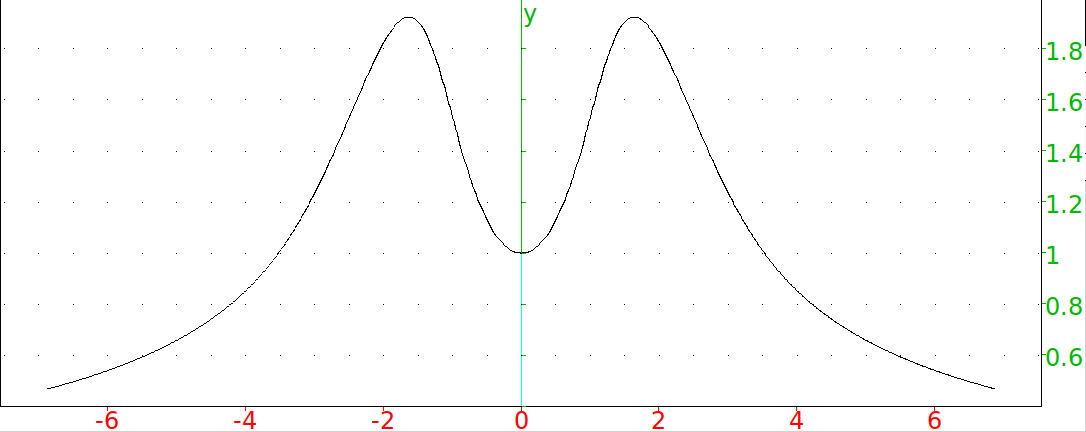
\includegraphics[width=\textwidth]{xcas-plotode.png}
\end{center}
The \texttt{plotfield} command will plot the entire vector field;
\xcasin{plotfield(sin(x*y),[x,y])}
will result in
\begin{center}
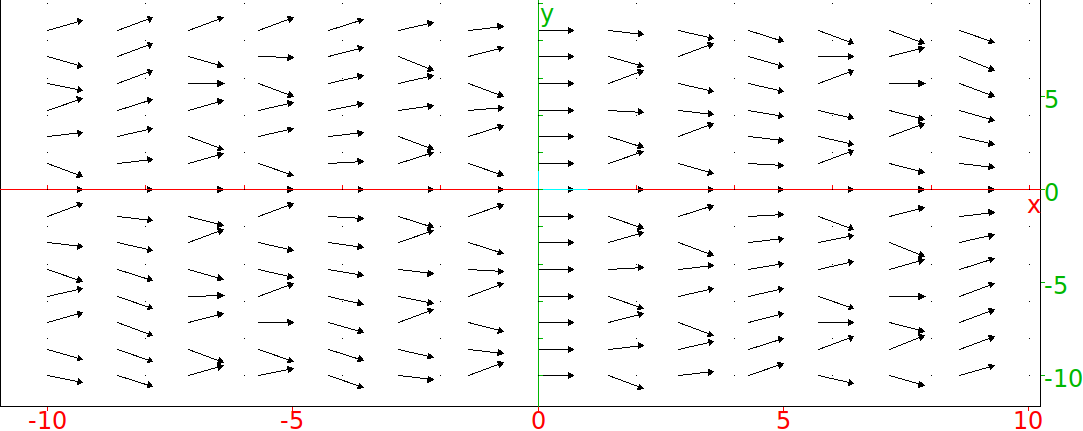
\includegraphics[width=\textwidth]{xcas-plotfield.png}
\end{center}
If you use the \texttt{interactive\_odeplot} command, you will get the
vector field and you will be able to click on a point to find the
graph of the solution passing through the point.


\section{Algebra with \texttt{Xcas}}

\subsection{Integer arithmetic}

\begin{center}
\begin{tabular}{|p{.25\textwidth}|p{.55\textwidth}|}
\hline
\multicolumn{2}{|c|}{\textbf{Integers}}\\
\hline\hline
\texttt{a\%p} & $a$ modulo $p$\\
\texttt{powmod(a,n,p)} & $a^n$ modulo $p$\\
\texttt{irem} & remainder\\
\texttt{iquo} & quotient\\
\texttt{iquorem} & quotient and remainder\\
\hline
\texttt{ifactor} & prime factorization\\
\texttt{ifactors} & list of prime factors\\
\texttt{idivis} & list of divisors\\
\hline
\texttt{gcd} & greatest common divisor\\
\texttt{lcm} & least common multiple\\
\texttt{iegcd} & Bezout's identity\\
\hline
\texttt{isprime} & primality test\\
\texttt{nextprime} & next prime number\\
\texttt{previousprime} & previous prime number\\
\hline
\end{tabular}
\end{center}
\index{powmod@{\texttt{powmod}}}
\index{irem@{\texttt{irem}}}
\index{remainder}
\index{iquo@{\texttt{iquo}}}
\index{quotient}
\index{iquorem@{\texttt{iquorem}}}
\index{ifactor@{\texttt{ifactor}}}
\index{prime factors}
\index{ifactors@{\texttt{ifactors}}}
\index{idivis@{\texttt{idivis}}}
\index{gcd@{\texttt{gcd}}}
\index{lcm@{\texttt{lcm}}}
\index{iegcd@{\texttt{{egcd}}}}
\index{Bezout}
\index{isprime@{\texttt{isprime}}}
\index{number!prime}
\index{nextprime@{\texttt{nextprime}}}
\index{previousprime@{\texttt{previousprime}}}

\texttt{Xcas} has the usual number theoretic functions.  The
\texttt{iquo} command will find the integer quotient of two integers
and \texttt{irem} will find the remainder.  The \texttt{iquorem}
command will return a list of both the quotient and remainder; if you
enter
\xcasin{iquorem(30,7)}
you will get
\xcasout{[4,2]}
since $30$ divided by $7$ is $4$ with a remainder of $2$.

The \texttt{gcd} and \texttt{lcm} commands will find the greatest
common divisor and least common multiple of two integers.  If you enter
\xcasin{gcd(72,120)}
returns 
\xcasout{24}
The greatest common divisor $d$ of two integers $a$ and $b$ can always be
written in the form $a*u + b*v = d$ for integers $u$ and $v$.  (This
is known as B\'ezout's Identity).  The \texttt{iegcd} will
return the coefficients $u$ and $v$ as well as the greatest commond
divisor.  If you enter
\xcasin{iegcd(72,120)}
you will get
\xcasout{[2,-1,24]}
since
\[ 72\cdot 2 + 120\cdot(-1) = 24\]

The \texttt{ifactor} command will give the prime factorization of an
integer; if you enter
\xcasin{ifactor(250)}
you will get
\xcasout{2*5^3}
You can use \texttt{ifactors} to get a list of the prime factors of an
integer, where in the list each factor is followed by its multiplicity.
If you enter
\xcasin{ifactors(250)}
you will get
\xcasout{[2,1,5,3]}
since $250$ has a prime factor of $2$ (it has $1$ factor of $2$) and a
prime factor of $5$ (it has $3$ factors of $5$).
The \texttt{idivis} command will return a complete list of factors;
\xcasin{idivis(250)}
will return
\xcasout{[1,2,5,10,25,50,125,250]}

The subject of primes is a difficult one, and you should see the
manual for a discussion of how \texttt{Xcas} checks for primes.  But
the command \texttt{isprime} will return \texttt{true} or \texttt{false}
depending on whether or not you enter a prime.  If you enter
\xcasin{isprime(37)}
will return
\xcasout{true}
since $37$ is a prime number.  The commands \texttt{nextprime} and
\texttt{previousprime} will find the first prime after (or before) the
number that you give it; if you enter
\xcasin{nextprime(37)}
you will get
\xcasout{41}
since the first prime after $37$ is $41$.

Integers modulo $p$ are defined by putting \texttt{\% p} after them.
Once an integer modulo $p$ is defined, then any calculations done with
it are done in $\Z/p\Z$.  For example, if you define
\xcasin{a := 3 \% 5}
then
\xcasin{a*2}
will return
\xcasout{1 \% 5}
(since 6 mod 5 is reduced to 1 mod 5); 
\xcasin{1/a}
will return
\xcasout{2 \% 5}
etc.  The \texttt{powermod} or \texttt{powmod} functions can be used
to efficiently calculate powers modulo a number.


\subsection{Polynomials and rational functions}

\begin{center}
\begin{tabular}{|p{.25\textwidth}|p{.55\textwidth}|}
\hline
\multicolumn{2}{|c|}{\bf Polynomials}\\
\hline\hline
\texttt{normal} & normal form (expanded and reduced)\\
\texttt{expand} & expanded form\\
\texttt{ptayl} & Taylor form\\
\texttt{peval} or \texttt{horner} & evaluation using Horner's method\\
\texttt{canonical\_form} & canonical form for a trinomial\\
\hline
\texttt{coeff} & list of coefficients\\
\texttt{poly2symb} & transform an algebraic polynomial to list form\\
\texttt{symb2poly} & transform the list form of a polynomial to
algebraic form\\
\texttt{pcoeff} & return the polynomial (list form) given a list of zeroes\\
\hline
\texttt{degree} & degree\\
\texttt{lcoeff} & the coefficient of the leading term\\
\texttt{valuation} & the lowest degree of the terms\\
\texttt{tcoeff} & the coefficient of the term with the lowest degree\\
\hline
\texttt{factor} & prime factorization\\
\texttt{factors} & list of prime factors\\
\texttt{divis} & list of divisors\\
\hline
\texttt{froot} & roots with multiplicities\\
\texttt{proot} & approximate values of the roots\\
\texttt{sturmab} & the number of roots in an interval\\
\hline
\texttt{getNum} & the numerator of a rational function\\
\texttt{getDenom} & the denominator of a rational function\\
\texttt{propfrac} & writes a rational expression as a whole part and a
proper rational part\\
\texttt{partfrac} & partial fraction decomposition\\
\hline
\texttt{quo} & quotient\\
\texttt{rem} & remainder\\
\texttt{gcd} & greatest common divisor\\
\texttt{lcm} & least common multiple\\
\texttt{egcd} & Bezout's identity
\\
\texttt{divpc} & Taylor polynomial for a rational expression\\
\hline
\texttt{randpoly} & random polynomial\\
\texttt{cyclotomic} & cyclotomic polynomial\\
\texttt{lagrange} & Lagrange polynomials\\
\texttt{hermite} & Hermite polynomials\\
\texttt{laguerre} & Laguerre polynomials\\
\texttt{tchebyshev1} & Tchebyshev polynomials\\
\texttt{tchebyshev2} & Tchebyshev polynomials\\
\hline
\end{tabular}
\end{center}
\index{normal@{\texttt{normal}}}
\index{expand@{\texttt{expand}}}
\index{ptayl@{\texttt{ptayl}}}
\index{polynomial!Taylor}
\index{Taylor polynomial}
\index{peval@{\texttt{peval}}}
\index{horner@{\texttt{horner}}}
\index{canonical\_form@{\texttt{canonical\_form}}}
\index{coeff@{\texttt{coeff}}}
\index{poly2symb@{\texttt{poly2symb}}}
\index{symb2poly@{\texttt{symb2poly}}}
\index{pcoeff@{\texttt{pcoeff}}}
\index{degree@{\texttt{degree}}}
\index{lcoeff@{\texttt{lcoeff}}}
\index{valuation@{\texttt{valuation}}}
\index{tcoeff@{\texttt{tcoeff}}}
\index{factor@{\texttt{factor}}}
\index{factors@{\texttt{factors}}}
\index{divis@{\texttt{divis}}}
\index{divisors}
\index{froot@{\texttt{froot}}}
\index{proot@{\texttt{proot}}}
\index{sturmab@{\texttt{sturmab}}}
\index{getNum@{\texttt{getNum}}}
\index{getDenom@{\texttt{getDenom}}}
\index{propfrac@{\texttt{propfrac}}}
\index{partfrac@{\texttt{partfrac}}}
\index{quo@{\texttt{quo}}}
\index{rem@{\texttt{rem}}}
\index{gcd@{\texttt{gcd}}}
\index{lcm@{\texttt{lcm}}}
\index{egcd@{\texttt{egcd}}}
\index{Bezout's identity}
\index{divpc@{\texttt{divpc}}}
\index{randpoly@{\texttt{randpoly}}}
\index{cyclotomic@{\texttt{cyclotomic}}}
\index{polynomial!cyclotomic}
\index{lagrange@{\texttt{lagrange}}}
\index{polynomial!Lagrange}
\index{hermite@{\texttt{hermite}}} 
\index{polynomial!Hermite}
\index{laguerre@{\texttt{laguerre}}}
\index{polynomial!Laguerre}
\index{tchebyshev1@{\texttt{tchebyshev1}}}
\index{polynomial!Tchebyshev}
\index{tchebyshev2@{\texttt{tchebyshev2}}}

Various polynomial operations are available in the \texttt{Polynomials}
submenu of the \texttt{Cmds} menu.

The \texttt{expand} or \texttt{normal} operators will distribute
multiplication across addition, and so expand a polynomial completely
out.  If you enter
\xcasin{expand((x+1)*(x+2)\^{}2)}
you will get
\xcasout{x^3+5*x^2+8*x+4}
Additionally, \texttt{normal} will reduce a rational expression to
lowest terms; if you enter
\xcasin{normal((x-1)\^{}2/(x\^{}2-1))}
you will get
\xcasout{\frac{x-1}{x+1}}

The \texttt{normal} operator will additionally put a rational
expression into lowest terms.  

The \texttt{factor} operator will factor a polynomial.  
If you enter
\xcasin{factor(x\^{}3+6*x\^{}2+3*x-10}
you will get
\xcasout{(x-1)*(x+2)*(x+5)}
The result often depends on the number field being used.  For example, over the
rational numbers the polynomial $x^4 - 1$ factors as 
$(x-1)(x+1)(x^2 + 1)$, while over the complex numbers it factors as 
$(x-1)(x+1)(x-i)(x+i)$.  If the coefficients of a polynomial are exact
fractions, then the factoring will be over the rationals.  To factor
over the complex numbers, you can configure \texttt{Xcas} to do
complex factorization (see section \ref{config}, ``Configuration'')
or use the \texttt{cfactor} command.
If the coefficients are in $\Z/p\Z$ then the polynomial will be
factored over  $\Z/p\Z$.


\subsection{Trigonometry}

\begin{center}
\begin{tabular}{|p{.20\textwidth}|p{.6\textwidth}|}
\hline
\multicolumn{2}{|c|}{\bf Trigonom\'etrie}\\
\hline\hline
\texttt{tlin} &linearize\\
\texttt{tcollect} & linearize and regroup\\
\texttt{texpand} & expand\\
\texttt{trig2exp} & trigonometric to exponential\\
\texttt{exp2trig} &exponential to trigonometric\\
\texttt{hyp2exp} &hyperbolic to exponential\\
\hline
\end{tabular}
\end{center}
\index{tlin@{\texttt{tlin}}}
\index{tcollect@{\texttt{tcollect}}}
\index{texpand@{\texttt{texpand}}}
\index{trig2exp@{\texttt{trig2exp}}}
\index{exp2trig@{\texttt{exp2trig}}}
\index{hyp2exp@{\texttt{hyp2exp}}}

\texttt{Xcas} has the usual trigonometic functions, both circular and
hyperbolic, as well as their inverses.  It also has commands for
manipulating trigonometric expressions; these are in the
\texttt{Trigo} submenus of the \texttt{Expression} menu.

One example is the \texttt{tlin} command will write products and powers of sines and
cosines as linear combinations of $\sin(n x)$s and $\cos(n x)$s.  If
you enter
\xcasin{tlin(2*sin(x)\^{}2*cos(3*x))}
you will get
\xcasout{-\frac{\cos(x)}{2} + \cos(3*x) - \frac{\cos(5*x)}{2}}

The \texttt{texpand} command will take expressions involving 
$\sin(n x)$ and $\cos(n x)$ and write them in terms of powers if
$\sin(x)$ and $\cos(x)$.  If you enter
\xcasin{texpand(sin(2*x)\^{}2*cos(3*x))}
you will get
\xcasout{16*\cos(x)^5*\sin(x)^2-12*\cos(x)^3*\sin(x)^2}


\subsection{Vectors and matrices}

\begin{center}
\begin{tabular}{|p{.20\textwidth}|p{.6\textwidth}|}
\hline
\multicolumn{2}{|c|}{\bf Vectors and matrices}\\
\hline\hline
\texttt{v*w} & scalar product\\
\texttt{cross(v,w)} & cross product\\
\texttt{A*B} & matrix product\\
\texttt{A.*B} & term by term product\\
\texttt{1/A} & inverse\\
\texttt{tran}& transpose\\
\texttt{rank} & rank\\
\texttt{det} & determinant\\
\texttt{ker} & basis for the kernel\\
\texttt{image} & base for the image\\
\texttt{idn} & identity matrix\\
\texttt{ranm} & matrix with random coefficients\\
\texttt{makematrix} & make a matrix from a function\\
\texttt{matrix} & make a matrix from a function\\
\texttt{blockmatrix} & combine matrices\\
\hline
\end{tabular}
\end{center}
\index{product!scalar}
\index{product!cross}
\index{product!matrix}
\index{product!term by term}
\index{rank@{\texttt{rank}}}
\index{det@{\texttt{det}}}
\index{ker@{\texttt{ker}}}
\index{image@{\texttt{image}}}
\index{idn@{\texttt{idn}}}
\index{ranm@{\texttt{ranm}}}
\index{matrix@{\texttt{matrix}}}
\index{makematrix@{\texttt{makematrix}}}
\index{blockmatrix@{\texttt{blockmatrix}}}
\index{matrix!identity}
\index{matrix!rank}
\index{matrix!kernel}
\index{matrix!image}
\index{matrix!determinant}
\index{determinant}

A vector is a list of numbers, such as \texttt{[2,3,5]}, and a matrix
is a list of vectors all of the same length, such as
\texttt{[[1,2,3],[4,5,6]]}.

The usual matrix operations (addition, scalar multiplication, matrix
multiplication) are done with the usual operators \texttt{+} and
\texttt{*}.  If you define
\xcasin{A := [[1,2,3],[4,5,6],[7,8,9]]}
\xcasin{B := [[1,1,1],[2,2,2]]}
then
\xcasin{3*A}
will give you
\xcasout{
\begin{pmatrix}
3 &   6 &  9\\
12 & 15 & 18\\
21 & 24 & 27
\end{pmatrix}}
and
\xcasin{B*A}
will give you
\xcasout{
\begin{pmatrix}
12 & 15 & 18\\
24 & 30 & 36
\end{pmatrix}}
A vector can be regarded as a matrix with one row, except that if a matrix
is multiplied on the right by a vector, the vector will be regarded as
a column.  In particular, if \texttt{v} and \texttt{w} are vectors of
the same length, then \texttt{v*w} returns the scalar product.

The \texttt{idn} command will create an identity matrix;
\xcasin{idn(2)}
will return
\xcasout{
\begin{pmatrix}
1 & 0\\
0 & 1
\end{pmatrix}}
You can also use \texttt{makemat} or \texttt{matrix} commands to build
a matrix. They both require a real-valued function of two variables,
the number of rows and the number of columns.  The indices start at 0,
and with the \texttt{makemat} the function comes first, with
\texttt{matrix} the function comes last.  Both
\xcasin{makemat((j,k)->j+k,3,2)}
and
\xcasin{matrix(3,2,(j,k)->j+k)}
produce
\xcasout{
\begin{pmatrix}
0 & 1\\
1 & 2\\
2 & 3
\end{pmatrix}}

Several matrices can be combined into a larger matrix with the
\texttt{blockmatrix} command.  To arrange $m * n$ matrices
into $m$ rows and $n$ columns, you give \texttt{blockmatrix} the
values $m$, $n$ and a list of the matrices.  If you enter
\xcasin{A := [[1,2,3],[4,5,6]]}
\xcasin{B := [[1,2],[2,3]]}
then
\xcasin{blockmatrix(2,2,[A,B,B,A])}
will give you
\xcasout{
\begin{pmatrix}
1 & 2 & 3 & 1 & 2\\
4 & 5 & 6 & 2 & 3\\
1 & 2 & 1 & 2 & 3\\
2 & 3 & 4 & 5 & 5
\end{pmatrix}}

You can get the elements from a matrix by following the matrix with
the indices in brackets, separated by commas.  For \texttt{A} as above,
\xcasin{A[1,2]}
will return
\xcasout{6}
You can extract a submatrix by using intervals of indices (the
beginning and end index separated by two periods);
\xcasin{A[0..1,1..2]}
returns
\xcasout{
\begin{pmatrix}
2 & 3\\
5 & 6
\end{pmatrix}}

Note that if you change one value of a matrix in \texttt{Xcas}, the
entire matrix will be copied.  If a program modifies parts of a large
matrix one element at a time, this time can add up.


\subsection{Linear systems}

\begin{center}
\begin{tabular}{|p{.20\textwidth}|p{.6\textwidth}|}
\hline
\multicolumn{2}{|c|}{\bf Linear systems}\\
\hline\hline
\texttt{linsolve} & solution of a linear system\\
\texttt{simult} & solutions of many linear systems\\
\texttt{rref} & Gauss-Jordan reduction\\
\hline
\end{tabular}
\end{center}
\index{Gauss-Jordan}
\index{linsolve@{\texttt{linsolve}}}
\index{simult@{\texttt{simult}}}
\index{rref@{\texttt{rref}}}

The \texttt{linsolve} command will solve a system of linear equations;
its syntax is the same as that of \texttt{solve} (see section
\ref{solve}, ``Solving equations'').
If you enter
\xcasin{linsolve([2*x + 3*y = 4, 5*x + 4*y = 3],[x,y])}
you will get
\xcasout{[-1,2]}

The \texttt{simult} command can also solve a system of linear
equations; more generally, it can solve several systems with the same
coefficient matrix.  To solve the systems
\[ A\mathbf{x} = \mathbf{b}_1,\dots,A\mathbf{x}=\mathbf{b}_k\]
you can enter
\xcasin{simult(A,B)}
where
\[ B = \left(\mathbf{b}_1 \cdots \mathbf{b}_k\right)\]
The result will be a matrix whose $j$th column is the solution of
$A\mathbf{x}=\mathbf{b}_j$.
For example, if you want to solve the systems
\[
\left\{ \begin{array}{llllllr}
 x &+& y &-& z&=&1\\
 x & -&  y&+& z&=&1 \\
 -x & +&y &+& z&=&-2 
\end{array}\right.
\]
\[
\left\{ \begin{array}{llllllr}
 x &+& y &-& z&=&-2\\
 x & -&  y&+& z&=&1 \\
 -x & +&y &+& z&=&1 
\end{array}\right.
\]
which both have the same matrix of coefficients
\[
\begin{pmatrix}
  1 & 1 & -1\\
  1 & -1 & 1\\
  -1 & 1 & 1
\end{pmatrix}
\]
you can create the matrix which has one column for each system
\[
\begin{pmatrix}
  1 & -2\\
  1 &  1\\
  -2 & 1
\end{pmatrix}
\]
If you enter
\xcasin{simult([[1,1,-1],[1,-1,1],[-1,1,1]],[[1,-2],[1,1],[-2,1]])}
you will get
\xcasout{
\begin{pmatrix}
1 & -1/2\\
-1/2 & -1/2\\
-1/2 & 1
\end{pmatrix}}
The solution to the first system is the first column,
$x=1,y=-1/2,z=-1/2$, and the solution to the second system is the
second column, $x=-1/2,y=-1/2,z=1$.

When there are no solutions, \texttt{linsolve} will return the empty
list while \texttt{simult} will return an error.  When there are
infinitely many solutions, \texttt{linsolve} will return formulas for
all solutions while \texttt{simult} will return one solution.

\subsection{Matrix reduction}

\begin{center}
\begin{tabular}{|p{.20\textwidth}|p{.6\textwidth}|}
\hline
\multicolumn{2}{|c|}{\textbf{Matrix reduction}}\\
\hline\hline
\texttt{jordan} & diagonalization or Jordan reduction\\
\texttt{pcar} & characteristic polynomial (list form)\\
\texttt{pmin} & minimal polynomial (list form)\\
\texttt{eigenvals} & eigenvalues\\
\texttt{eigenvects} & eigenvectors\\
\hline
\end{tabular}
\end{center}
\index{jordan@{\texttt{jordan}}}
\index{Jordan form}
\index{diagonalization}
\index{pcar@{\texttt{pcar}}}
\index{pmin@{\texttt{pmin}}}
\index{eigenvals@{\texttt{eigenvals}}}
\index{eigenvects@{\texttt{eigenvects}}}
\index{polynomial!characteristic}
\index{polynomial!minimal}
\index{eigenvalues}
\index{eigenvectors}

The \texttt{jordan} command will take a matrix $A$ and returns a
transition matrix $P$ and a matrix $J$ in Jordan canonical form such
that $P^{-1} A P = J$.  In particular, if $A$ is diagonalizable, then
$J$ will be diagonal with the eigenvalues of $A$ on the diagonal and
the columns of $P$ will be the corresponding eigenvectors.
If you enter
\xcasin{jordan([[4,1],[-8,-5]])}
you will get
\xcasout{
\left(\begin{pmatrix}1 & 1\\ -1 & -8 \end{pmatrix},
      \begin{pmatrix}3 & 0\\ 0 & -4 \end{pmatrix}\right)}
This means that $3$ and $-4$ (the diagonal elements of the second
matrix) are the eigenvalues of 
$\begin{pmatrix}4 & 1\\-8 & -5\end{pmatrix}$ and the corresponding
eigenvectors are $\begin{pmatrix}1\\-1\end{pmatrix}$ and
$\begin{pmatrix}1\\-8\end{pmatrix}$ (the columns of the first matrix).
For diagonalizable matrices you can also get this information with the
\texttt{eigenvals} and \texttt{eigenvects} commands;
\xcasin{eigenvals([[4,1],[-8,-5]])}
will return
\xcasout{(3,-4)}
and 
\xcasin{eigenvects([[4,1],[-8,-5]])}
will return
\xcasout{\begin{pmatrix}1 & 1\\ -1 & -8 \end{pmatrix}}

For matrices with exact and symbolic values, the only eigenvalues used
are those computable with \texttt{solve}; for matrices with floating
point numbers, a numerical algorithm is used to find the eigenvalues.
This algorithm may fail in some cases where there are very close
eigenvalues or eigenvalues with multiplicity greater than one.

If a function is defined by a polynomial, you can evaluate it with an
argument of a square matrix.  If a function is given by a series, the
Jordan form of the matrix can be used to define the value of the
function at a matrix.  For example, you can find the exponential of a
square matrix;
\xcasin{exp([[0,-1],[1,2]])}
results in
\xcasout{
\begin{pmatrix}
0 & -\exp(1)\\
\exp(1) & 2*\exp(1)
\end{pmatrix}}


\section{Graphs}

\begin{center}
\begin{tabular}{|p{.20\textwidth}|p{.6\textwidth}|}
\hline
\multicolumn{2}{|c|}{\bf Plotting graphs}\\
\hline\hline
\texttt{plot} & graph an expression of one variable\\
\texttt{plotfunc} & graph an expression of one or two variables\\
\texttt{tangent} & tangent to a curve\\
\texttt{plotparam} & parametric curve\\
\texttt{plotpolar} & polar plotting\\
\texttt{plotimplicit} & implicit curve\\
\hline
\end{tabular}
\end{center}
\index{plot@{\texttt{plot}}}
\index{plotfunc@{\texttt{plotfunc}}}
\index{tangent@{\texttt{tangent}}}
\index{plotparam@{\texttt{plotparam}}}
\index{plopolar@{\texttt{plotpolar}}}
\index{plotimplicit@{\texttt{plotimplicit}}}
\index{curve!parametric}
\index{curve!polar}
\index{curve!implicit}

The \texttt{Graphic} menu has entries for several graphing commands;
if you choose one you will be given a template you can fill out to
produce a graphic.  The appropriate command will be placed on the
command line.  If you want several graphs in the same window, you can
put the commands on the same command line separated by semicolons.

Once you have created a graphic window, there will be a panel to the
right with buttons allowing you to control the image.  The default
parameters for graphs, such as the size of the graphs, are
configurable (see section \ref{config}, ``Configuration'').

As well as being displayed in the \texttt{Xcas} window, the two
dimensional graphics also appear in the DispG (Display Graphics)
window.  You can bring that window up with the
\texttt{Cfg$\blacktriangleright$Show$\blacktriangleright$DispG} menu item.
This window will contain all two dimensional graphs; they can be
cleared with the \texttt{ClrGraph} command. 

\subsection{Curves}

The simplest way to draw graphs is with the templates from the
\texttt{Graphic} menu, but there are command line equivalents. 

The command line instruction for graphing a function is the
\texttt{plot} command.  It takes an expression (or list of
expressions) followed by the variable.  To use a domain different than
the default, you can indicate the range of the variable by setting it
equal to an interval.  If you are plotting several curves, you can
distinguish them by giving them different colors; you can do this with
a third argument \texttt{color=} followed by a list of colors.
If you plot
\xcasin{plot([x\^{}2,x\^{}3],x=-1..1,color=[red,blue])}
you will get
\begin{center}
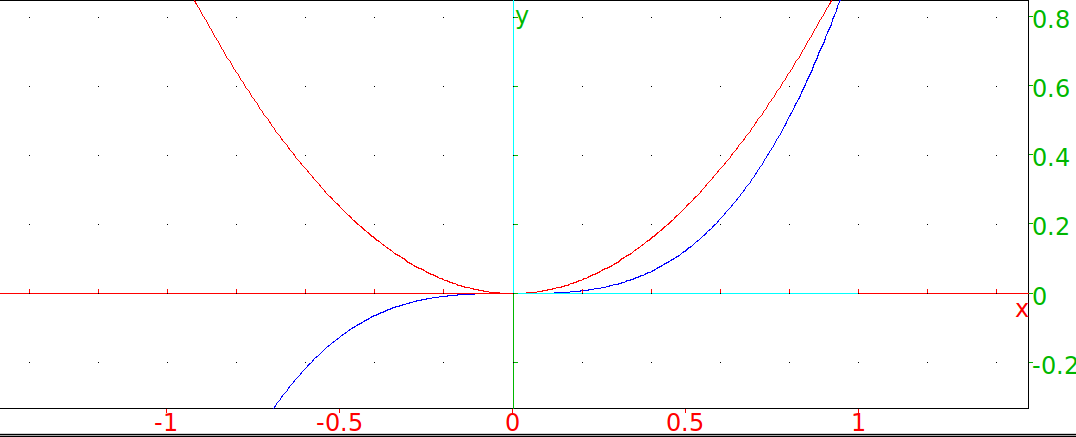
\includegraphics[width=\textwidth]{xcas-plot.png}
\end{center}

You can draw parameterized curves with the \texttt{plotparam} command.
The coordinates of the curve must be given as a single complex
expression; the $x$ coordinate will be the real part of the expression
and the $y$ coordinate will be the imaginary part.  For example, if
you enter
\xcasin{plotparam(sin(t) + i*cos(t),t)}
you will get the circle
\begin{center}
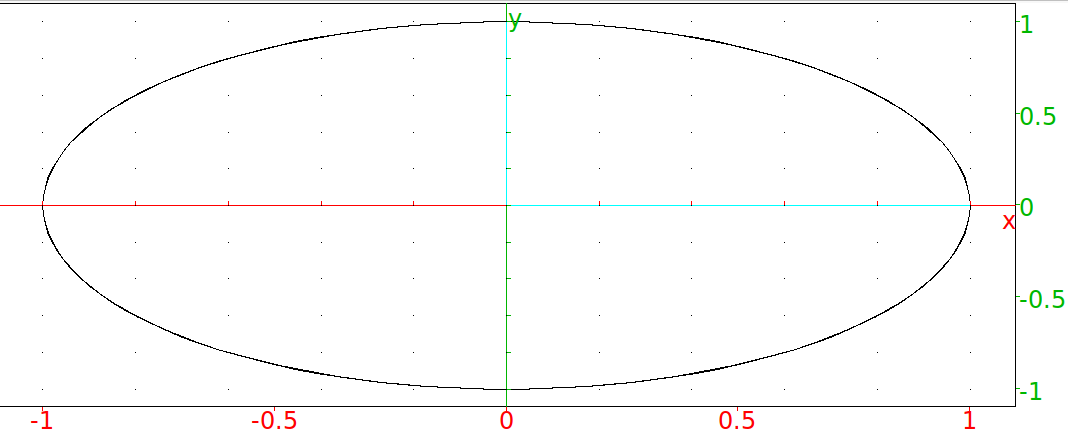
\includegraphics[width=\textwidth]{xcas-plotparam.png}
\end{center}
(Since the $x$- and $y$-axes are scaled differently, the circle
looks elliptical.)

You can draw a curve using polar coordinates with the
\texttt{plotpolar} command.  This takes the form
\texttt{plotpolar(f(theta),theta,theta-min,theta-max)}.

You can draw an implicitly defined curve with the
\texttt{plotimplicit} command; the command
\texttt{plotimplicit($f(x,y)$,$x$,$y$)} will draw the curve
$f(x,y)=0$.  For example, the command
\xcasin{plotimplicit(x\^{}2 + y\^{}2 = 1,x,y)}
will draw a circle.

The \texttt{tangent} command will draw the tangent line to a curve, if
you tell it the curve and the point.  To draw the tangent line to the
graph $y=x^2$ at $x=1$, for example, you can enter
\xcasin{tangent(plotfunc(x\^{}2,x),1)}
You will get
\begin{center}
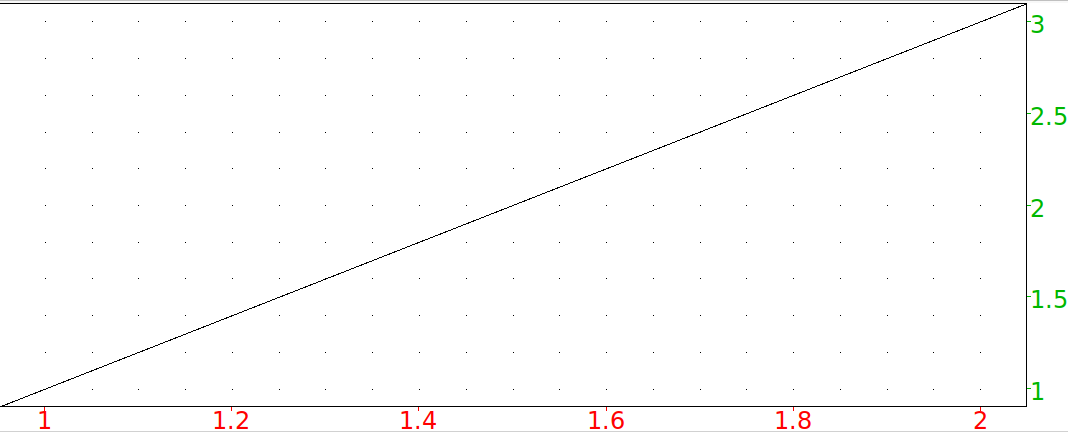
\includegraphics[width=\textwidth]{xcas-tangent.png}
\end{center}


\subsection{Plane geometry}

\begin{center}
\begin{tabular}{|p{.20\textwidth}|p{.6\textwidth}|}
\hline
\multicolumn{2}{|c|}{\bf 2D graphical objects}\\
\hline\hline
\texttt{legend} & place text starting from a given point\\
\texttt{point} & determine a point given a complex number or two
coordinates\\
\texttt{segment} & segment determined by 2 points\\
\texttt{circle} & circle determined by a point and radius\\
\texttt{inter} & find the intersection of curves\\
\texttt{equation} & return the cartesian equation of a curve\\
\texttt{parameq} & return the parametric equation of a curve\\
\texttt{polygonplot} & draw a polygonal line\\
\texttt{scatterplot} & draw a cloud of dots\\
\texttt{polygon} & draw a closed polygon\\
\texttt{open\_polygon} & draw an open polygon\\
\hline
\end{tabular}
\end{center}
\index{legend@{\texttt{legend}}}
\index{text}
\index{point@{\texttt{point}}}
\index{segment@{\texttt{segment}}}
\index{circle@{\texttt{circle}}}
\index{inter@{\texttt{inter}}}
\index{equation@{\texttt{equation}}}
\index{intersection}
\index{polygonal line}
\index{polygonplot@{\texttt{polygonplot}}}
\index{polygon@{\texttt{polygon}}}
\index{open\_polygon@{\texttt{open\_polygon}}}
\index{cloud of dots}
\index{circle@{\texttt{circle}}}
\index{equation@{\texttt{equation}}}
\index{parameq@{\texttt{parameq}}}
\index{scatterplot@{\texttt{scatterplot}}}

Among its other capabilities, \texttt{Xcas} works with plane geometry.
The \texttt{Geo$\blacktriangleright$New figure 2D} menu item or the
\texttt{Alt+g} key will bring up the screen for plane geometry.

A point on the geometry screen can be specified with the
\texttt{point} command, which can take either an ordered pair or real
numbers or a complex number as argument.  The \texttt{Geo} menu
contains many commands for drawing geometric objects, such as
\texttt{circle} (which takes a point and a radius as arguments) and
\texttt{polygon} (which takes a sequence of points as arguments).

Some functions, such as \texttt{polygonplot} and \texttt{scatterplot},
take lists of $x$-coordinates and $y$-coordinates as arguments.  For
example,
\xcasin{polygonplot([0,2,0],[0,0,2])}
and 
\xcasin{open\_polygon(point(0,0),point(2,0),point(0,2))}
will both draw the same segments.

The \texttt{legend} can be used to place text on the screen; one
simple way of using it is to give it a point and text as arguments.


\subsection{3D graphical objects}

\begin{center}
\begin{tabular}{|p{.20\textwidth}|p{.6\textwidth}|}
\hline
\multicolumn{2}{|c|}{\textbf{3D graphical objects}}\\
\hline\hline
\texttt{plotfunc} & graph of a function\\
\texttt{plotparam} & parametric surface\\
\hline\hline
\texttt{point} & point\\
\texttt{plane} & plane\\
\texttt{sphere} & sphere with a center and radius\\
\texttt{cone} & cone with a center, axis and opening angle\\
\texttt{inter} & intersection \\
\texttt{polygon} & polygon \\
\texttt{open\_polygon} & open polygon\\
\hline
\end{tabular}
\end{center}
\index{space}
\index{plotfunc@{\texttt{plotfunc}}}
\index{plotparam@{\texttt{plotparam}}}
\index{point@{\texttt{point}}}
\index{polygonal line}
\index{polygonplot@{\texttt{polygonplot}}}
\index{polygon@{\texttt{polygon}}}
\index{open\_polygon@{\texttt{open\_polygon}}}
\index{plane@{\texttt{plane}}}
\index{sphere@{\texttt{sphere}}}
\index{cone@{\texttt{cone}}}
\index{inter@{\texttt{inter}}}

\texttt{Xcas} can also handle three-dimensions graphically, either by
drawing curves and graphs in three-dimensions or by drawing
three-dimensional geometric objects.  A three-dimensional screen can
be brought up with the \texttt{Geo$\blacktriangleright$New figure 3D}
menu item or the \texttt{Alt+h} key.
There will controls for the view window to the right of the screen.
You can rotate the visualization cube by using the mouse outside of
the cube or by clicking in the cube and using the \texttt{x},
\texttt{y} and \texttt{z} keys to rotate and the \texttt{+} and
\texttt{-} keys for zooming.

You can draw a graph $z = f(x,y)$ with the \texttt{plotfunc} command,
which takes an expression and a list of two variables.  Like graphs of
functions of one variable, you can use a domain different than the
default by giving the variables their own intervals.  The command
\xcasin{plotfunc(y\^{}2 - x\^{}2,[x=-1..1,y=-1..1])}
will give you the graph
\begin{center}
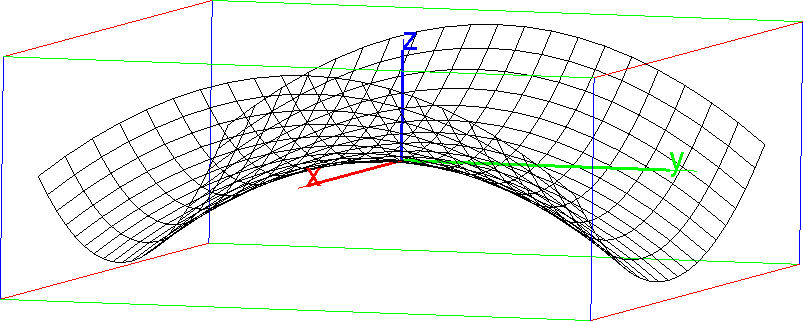
\includegraphics[width=\textwidth]{xcas-3dplot.png}
\end{center}

The \texttt{plotparam} command can be used to draw a parameterized
curves and surfaces in three-dimensions.  If the first argument is a
list of three expressions involving two variables and the next two
arguments are the variables (with optional intervals), then
\texttt{plotparam} will plot the surface.   If you enter
\xcasin{plotparam([u,u+v,v],u,v)}
you will get
\begin{center}
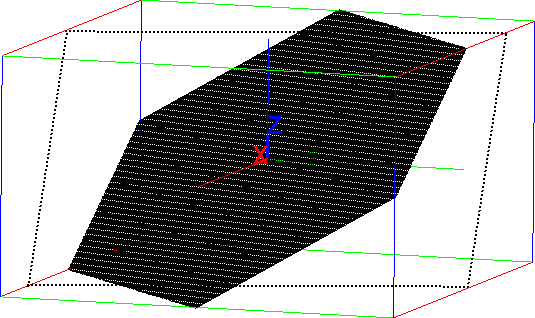
\includegraphics[width=\textwidth]{xcas-3dparam.png}
\end{center}
If the first argument is a list of three expressions involving one
variable and the next argument is the variable, then
\texttt{plotparam} will plot the curve.  If you enter
\xcasin{plotparam([cos(t),sin(t),t],t)}
you will get
\begin{center}
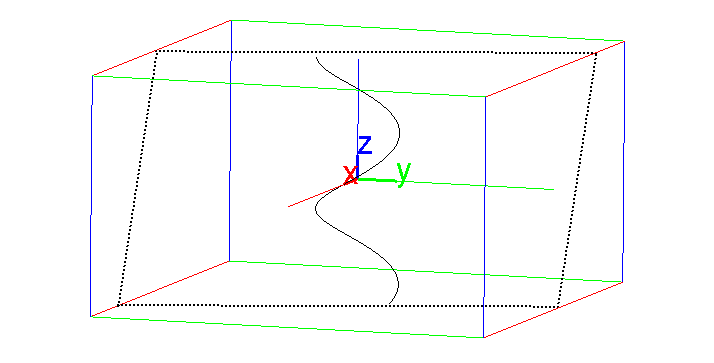
\includegraphics[width=\textwidth]{xcas-3dcurve.png}
\end{center}

A point in three-dimensions is given with the \texttt{point} command
with three arguments.  Commands like \texttt{polygon} and
\texttt{open\_polygon} work in three-dimensions as well as two, as
well as additional commands such as \texttt{sphere}.  A plane can be
drawn with the \texttt{plane} command, which can be given either three
points, a line and two points, or an equation of the form \texttt{a*x
+ b*y + c*z = d}.


\section{Programming}

\subsection{The language}

\begin{center}
\begin{tabular}{|p{.52\textwidth}|p{.28\textwidth}|}
\hline
\multicolumn{2}{|c|}{\textbf{Instructions for \texttt{Xcas}}}\\
\hline\hline
\texttt{a:=2;} & assignment \\
\texttt{input("a=",a);} & input expression \\
\texttt{textinput("a=",a);} & string input \\
\texttt{print("a=",a);} & output\\
\texttt{return(a);} & return value\\
\texttt{break;} & break out of loop\\
\texttt{continue;} & go to the next iteration\\
\texttt{if (<condition>) {<inst>};}  & if\dots then\\
\texttt{if (<condition>) {<inst1>} else {<inst2>};}  &
	     if\dots then \dots else\\
\texttt{for (j:= a;j<=b;j++) {<inst>};} & for loop\\
\texttt{for (j:= a;j<=b;j:=j+p) {<inst>};} & for loop\\
\texttt{repeat <inst> until <condition>;} & repeat loop\\
\texttt{while (<condition>) {<inst>};} & while loop\\
\texttt{do <inst1> if (<condition>) break;<inst2> od;} & do loop\\
\hline
\end{tabular}
\end{center}
\index{test}
\index{loops}
\index{if@{\texttt{if}}}
\index{else@{\texttt{else}}}

\begin{center}
\begin{tabular}{|p{.20\textwidth}|p{.6\textwidth}|}
\hline
\multicolumn{2}{|c|}{\bf Boolean operators}\\
\hline\hline
\texttt{==}   & test for equality\\
\texttt{!=} & test for inequality\\
\texttt{<}    & test for strictly less than\\
\texttt{>}  & test for strictly greater than\\
\texttt{<=}   & tes  for less than or equal\\
\texttt{>=} & test for greater than or equal to\\
\texttt{\&\&}, \texttt{and} & infixed ``and''\\
\texttt{||}, \texttt{or}& infixed ``or''\\
\texttt{true}    & boolean true (same as 1)\\
\texttt{false}  & boolean false (same as 0)\\
\texttt{not}, \texttt{!} & ``not''\\
\hline
\end{tabular}
\end{center}
\index{and}
\index{or}
\index{not}
\index{test}
\index{if@{\texttt{if}}}
\index{else@{\texttt{else}}}
\index{for@{\texttt{for}}}
\index{loop}

You can extend \texttt{Xcas} by adding desired functions with its
built-in programming language.  The  main features of the language are:

\begin{itemize}
  \item 
  It is a functional language.  The argument of a function can
  be another function; in which case you can either give the name of
  a function or the definition of the function.  If 
  \texttt{f(x) := x\^{}2}, then
  \texttt{function\_diff(f)} is the same as
  \texttt{function\_diff(x->x\^{}2)}.
  
  \item
  There is no distinction between a program and a function.  A
  function returns the value of the last evaluated statement or what
  follows the reserved word \texttt{return}.

  \item
  The language is untyped.  Any variable can take on any value; the
  only different types of variables are global variables, which are
  not declared, and local variables, which are declared at the
  beginning of a function.
\end{itemize}

A function declaration looks like
\begin{verbatim}
   function_name (var1, var2, ...) := {
   local var_loc1, var_loc2, ... ;
     statement1;
     statement2;
     ...
   }
\end{verbatim}
The syntax is similar to \texttt{C++}, although many variants are
recognized, particularly in compatibility mode.
Recall that \texttt{i} is $\sqrt{-1}$ and cannot be used for a loop
variable.  
The conditional tests are Booleans, which are the results of the usual
Boolean operators.

A program can capture runtime errors with a
\texttt{try}--\texttt{catch} construction, which takes the form
\begin{verbatim}
   try 
     {
      block to catch errors
     }
   catch (variable)
     {
      block to execute when an error is caught
     }
\end{verbatim}
For example, the following will catch an error caused by incorrect
matrix multiplication:
\begin{verbatim}
   try 
     { A := idn(2) * idn(3) }
   catch (error)
     { print("The error is " + error) }
\end{verbatim}

\subsection{Some examples}

To write a program, it is a good idea to use the program editor that
comes with \texttt{Xcas}, which provides a template and commands
helpful for writing programs.  You can open this editor with the
\texttt{New Program} item in the \texttt{Prg} menu or the
\texttt{Alt+p} key.

Consider the following program, which takes two integers and returns the
quotient and remainder of the Euclidean division algorithm (like the
\texttt{iquorem} function).
\begin{verbatim}
   idiv2(a,b) := {
     local q,r;
     if (b != 0) {
       q := iquo(a,b);
       r := irem(a,b);
       }
     else {
       q := 0;
       r := a;
       }
     return [q,r];
   }
\end{verbatim}
If you enter this into the editor, you can test it with the
\texttt{OK} button.  You can then use the function in the command
line; if you enter
\xcasin{idiv2(25,15)}
you will get
\xcasout{[1,10]}
You can save it in a file; the name \texttt{idiv2.cxx} would be a good
name.  You can then use it in later session with the command
\xcasin{read("idiv2.cxx")}
or opening it in the program editor and validating it with the
\texttt{OK} button.

Here are some more programs that you can play with.  This first one
computes the GCD of two integers iteratively.
\begin{verbatim}
   pgcdi(a,b) := {
     local r;
     while (b != 0) {
       r := irem(a,b);
       a := b;
       b := r;
       }
     return a;
   }:;
\end{verbatim}
The second one computes the GCD recursively.
\begin{verbatim}
   pgcdr(a,b) := {
     if (b == 0) return a;
     return pgcdr(b, irem(a,b));
   }:;
\end{verbatim}

If a program doesn't work the way you expect, you can run it in
step-by-step mode with the debug command.  For more details, consult
the \texttt{Interface} item of the \texttt{Help} menu.  For example,
you can start the debugging by typing
\xcasin{debug(idiv2(25,15))}
The debugger will automatically display the values of the parameters
\texttt{a} and \texttt{b} and local variables \texttt{q} and
\texttt{r} when executing the program line by line with the
\texttt{sst} button.

\subsection{Programming style}

The \texttt{Xcas} programming language is interpreted, not compiled.
The run time of an \texttt{Xcas} program is affected by the number of
instructions rather than the number of lines.  

The speed of a program does not always match up with the clarity of
the program; compromises are often necessary.  For the most part, the
calculation time isn't an issue; interpreted languages are often used
to test algorithms and create models.   Full scale applications are
written in a compiled language like \texttt{C++}.  A \texttt{C++} can
use \texttt{giac} for the formal calculations.

When you are trying to write a fast program, you may want to take into
account the number of instructions and the speed of the instructions.
For example, it is in general faster to create lists and sequences
than it is to program loops.  Recall than in \texttt{Xcas} you can
find out how long it takes to run a command by entering
\xcasin{time(\textit{command})}

\newpage

\printindex

\end{document}

\section{Exercises}

\subsection{Functions and graphs}

\noindent
\textbf{Exercise 1.}\\
Let $f:\R - \{3\} \to \R$ by
\[ f(x) = (x+1)\ln|x-3|\]
\begin{enumerate}
  \item
  Find the derivative $f'$ and the second derivative $f''$.
  \item
  Find the limit of $f'(x)$ as $x$ approaches negative infinity and as $x$
  approaches 3 from the left.
  \item
  Show that $f'$ vanishes once in $(-\infty,3)$.  Find an interval of
  width 0.1 containing the point where $f'$ vanishes.
  \item
  Determine the intervals on which $f(x)$ is increasing and the
  intervals on which it is decreasing.
  \item
  Plot the graph of $f(x)$.
  \item
  Find the area between the graph of $f$, the $x$-axis, and the lines
  $x=-1$ and $x=2$.
\end{enumerate}

\noindent
\texttt{Solutions}\\
\begin{enumerate}
  \item
  You can define $f$ by
  \xcasin{f(x) := (x+1)*ln(abs(x-3))}
  To find $f'$, you can enter
  \xcasin{f1 := function\_diff(f):;}
  Then
  \xcasin{f1(x)}
  will return
  \xcasout{\ln(|x-3|) + \frac{x+1}{x-3}}
  So
  \[ f'(x) = \ln(|x-3|) + \frac{x+1}{x-3}\]
  Next, to find $f''$, you can enter
  \xcasin{f2 := function\_diff(f1)}
  Then
  \xcasin{f2(x)}
  will return
  \xcasout{\frac{1}{x-3} - \frac{4}{(x-3)^2}}
  This can be tidied with
  \xcasin{factor(f2(x))}
  which returns
  \xcasout{\frac{x-7}{(x-3)^2}}
  
  Alternatively, once $f$ is defined as above, you can compute the
  expression
  \xcasin{dfx := diff(f(x),x)}
  to get
  \xcasout{\ln(|x-3|) + \frac{x+1}{x-3}}
  To define this as a function, you can enter
  \xcasin{f1 := unapply(dfx,x)}
  Next, to calculate $f''(x)$, you can enter
  \xcasin{ddfx := diff(dfx)}
  to get
  \xcasout{\frac{1}{x-3} - \frac{4}{(x-3)^2}}
  If you want a function for $f''$ you can define
  \xcasin{f2 := unapply(ddfx,x)}
  \item
  Since
  \xcasin{limit(f1(x),x,-infinity)}
  returns
  \xcasout{+\infty}
  we get
  \[\lim_{x\to -\infty} f'(x) = +\infty\]
  Since
  \xcasin{limit(f1(x),x,3,-1)}
  returns
  \xcasout{-\infty}
  we get
  \[\lim_{x\to 3^-} f'(x) = -\infty\]
  
  \item
  Since $f''(x) = (x-7)/(x-3)^2 < 0$ for $x$ in $(-\infty,3)$, the
  function $f'$ is decreasing as well as continuous from $-\infty$ to
  $3$.  From (2), you can see that $f'$ passes through all real values
  on $(-\infty,3)$, so $f'(x) = 0$ for a unique $x$ in $(-\infty,3)$.
  To approximate this value, you can enter
  \xcasin{assume(x<3); fsolve(f1(x),x)}
  which will return
  \xcasout{x, 0.776592890991}
  (You may wish to enter
  \xcasin{purge(x)}
  to remove the hypothesis on $x$.)
  Since
  \xcasin{f1(0.7)}
  returns
  \xcasout{0.0937786881525}
  and
  \xcasin{f1(0.8)}
  returns
  \xcasout{-0.0297244578175}
  you know that $f'(0.7) > 0$ and $f'(0.8) < 0$, so $f'(x) = 0$ for
  some $x$  in $(0.7,0.8)$.
  
  \item
  On the interval $(3,\infty)$, $f''(x)$ is positive for $x>7$ and
  negative for $x < 7$.  That means that $f'(x)$ has a minimum at
  $x=7$.  Since 
  \xcasin{f1(7)}
  returns
  \xcasout{\ln(4)+2}
  the minimum value of $f'(x)$ on $(3,\infty)$ is positive, so $f'(x)
  > 0$ for all $x$ in $(3,\infty)$.  So $f(x)$ is increasing on
  $(3,\infty)$.
  
  Letting $\alpha$ be the solution of $f'(x) = 0$ in $(-\infty,3)$,
  you get that $f'(x) > 0$ for $x$ in $(-\infty,\alpha)$ and $f'(x) <
  0$ for $x$ in $(\alpha,3)$.  So $f(x)$ is increasing on
  $(-\infty,\alpha)$ and decreasing on $(\alpha,3)$.

  \item
  Entering
  \xcasin{plotfunc(f(x),x)}
  returns
  \begin{center}
  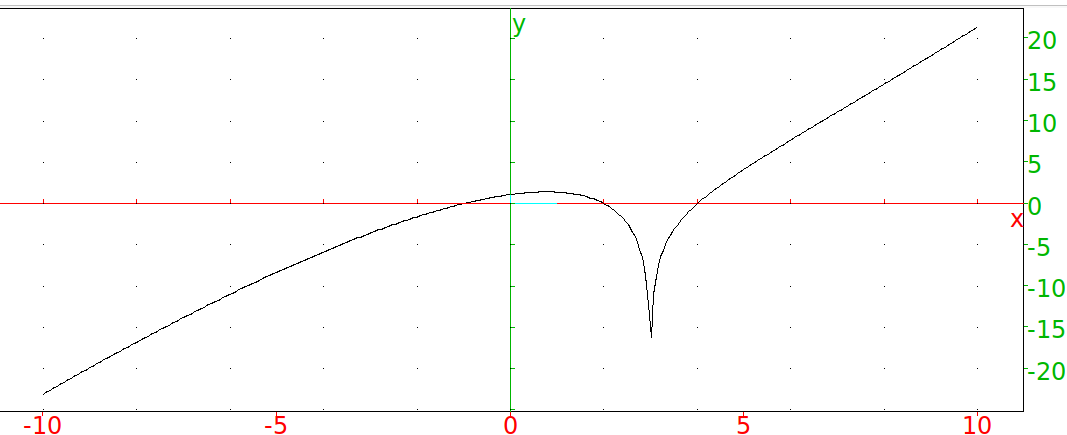
\includegraphics[width=\textwidth]{xcas-ex1.png}
  \end{center}
  You can note that this matches up with the information from (4).

  \item
  To find the area, you can enter
  \xcasin{integrate(f(x),x,-1,2)}
  giving you
  \xcasout{8*\ln(4) - \frac{33}{4}}
\end{enumerate}  

\noindent
\textbf{Exercise 2.}\\
Let $f:\R \to \R$ by
\[ f(x) = \frac{\exp(x)^2 - \exp(x) + 1}{\exp(x)^3 + \exp(x)}\]
\begin{enumerate}
  \item
  Show that for all $x \in \R$, $P(x) = x^4 - 2x^3 + 2x^2 + 1 \ge 1$.
  \item
  Determine where $f(x)$ is increasing, where it is decreasing, and
  plot the graph.
  \item
  Find the equation of the tangent line to the graph of $f$ at $x=0$.
  \item
  Calculate $\int_0^x f(t) dt$ and $\lim_{x\to + \infty} \int_0^x f(t)dt$.
\end{enumerate}

\noindent
\texttt{Solutions.}\\
\begin{enumerate}
  \item
  Entering
  \xcasin{factor(x\^{}4 - 2*x\^{}3 + 2*x\^{}2)}
  gives you
  \xcasout{x^2*(x^2 - 2*x + 2)}
  Working on the second factor,
  \xcasin{canonical\_form(x\^{}2-2*x + 2)}
  gives you
  \xcasout{(x-1)^2 + 1}
  So
  \[ x^4 - 2x^3 + 2x^2 = x^2(x-1)^2 + x^2 \ge 0\]
  and so for all $x \in \R$,
  \[ P(x) = x^4 - 2x^3 + 2x^2 + 1 \ge 1.\]

  \item
  Define
  \xcasin{f(x) := (exp(x)\^{}2 - exp(x) + 1)/(exp(x)\^{}3 + exp(x))}
  Computing \texttt{diff(f(x),x)} returns an overly complicated
  expression, which can be simplified with \texttt{normal}.  
  \xcasin{normal(diff(f(x),x))}
  gives you
  \xcasout{\frac{-\exp(x)^4+2*\exp(x)^3-2*\exp(x)^2-1}{\exp(x)^5+2*\exp(x)^3+\exp(x)}}
  Since the denominator is strictly positive and the numerator is
  $-P(\exp(x))$ which is always negative, you can see that $f'(x)$ is
  always negative, and so $f(x)$ decreases for all $x$.
  
  To get more information about the graph, note that
  \xcasin{limit(f(x),x=+infinity)}
  gives you
  \xcasout{0}
  and
  \xcasin{limit(f(x),x=-infinity)}
  gives you
  \xcasout{+\infty}.
  Plotting the graph with
  \xcasin{plotfunc(f(x),x)}
  gives you
  \begin{center}
  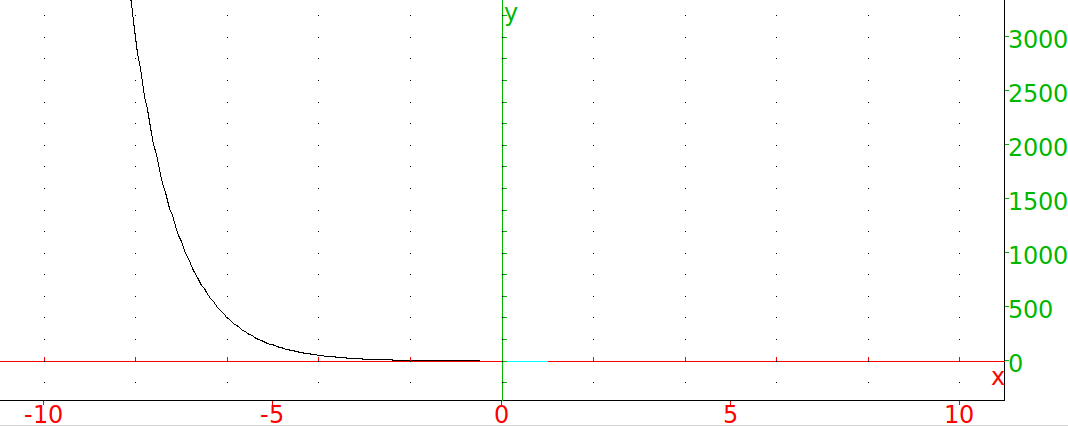
\includegraphics[width=\textwidth]{xcas-ex2.png}
  \end{center}
  which matches with the previous information.

  \item
  Since
  \xcasin{f(0)}
  returns 
  \xcasout{\frac{1}{2}}
  the tangent line will pass through $x=0, y=1/2$.
  To define the function $f'$, enter
  \xcasin{fprime := unapply(normal(diff(f(x),x)),x)}
  Since 
  \xcasin{fprime(0)}
  returns
  \xcasout{-\frac{1}{2}}
  the tangent line has slope  $f'(0) = -1/2$.
  The tangent line is then
  \[ y = f'(0)*x + f(0)\]
  which is
  \[ y = -\frac{1}{2} x + \frac{1}{2}\]
  
  \item
  To evaluate the integral, set
  \xcasin{intf := int(f(t),t,0,x)}
  giving you
  \xcasout{-\frac{ln(2)-2}{2}+\frac{-2*x*\exp(x)+\ln(\exp(x)^2+1)*\exp(x)-2}{2*exp(x)}}
  which is the integral.  To find the limit, enter
  \xcasin{limit(intf,x=+infinity)}
  which gives you
  \xcasout{-\frac{\ln(2)}{2} + 1}
\end{enumerate}


\subsection{Integrals}

\noindent
\textbf{Exercise 1.}\\
Evaluate
\[\int_1^2 \frac{1}{x^3 + 1} dx\]
\noindent
\texttt{Solution.}\\
Using \texttt{normal} to simplify the result, the integral is
\xcasin{normal(int(1/(x\^{}3 + 1),x,1,2))}
giving you
\xcasout{\frac{\sqrt{3}}{18}*\pi-\frac{1}{3}*\ln(2)+\frac{1}{6}*\ln(3)}

\noindent
\textbf{Exercise 2.}\\
Do a partial fraction decomposition of $t^2/(1-t^4)$.  Then evaluate
$\int t^2/(1-t^4)dt$ and $\int \sin^2(x)/\cos(2x) dx$.

\noindent
\texttt{Solution.}\\
To find the partial fraction decomposition, enter
\xcasin{partfrac(t\^{}2/(1-t\^{}4))}
giving you a decomposition of
\xcasout{-\frac{1}{(t-1)*4} +\frac{1}{(t+1)*4}-\frac{1}{(t^2+1)*2}}

To find the first integral, you can enter
\xcasin{int(t\^{}2/(1-t\^{}4),t)}
If you were doing it by hand you'd want to use the partial fraction
decomposition; letting the computer do it, you could enter
\xcasin{int(-1/((t-1)*4) + 1/((t+1)*4) - 1/((t\^{}2+1)*2), t)}
Either way, you will get
\xcasout{\frac{\ln(|t+1|)}{4} - {\ln(|t-1|)}{4} -
\frac{\mbox{atan}(t)}{2}}

To evaluate the second integral, you could do some substitutions to
turn it into the first integral; first write everything in terms of
tangents with
\xcasin{trigtan(texpand((sin(x)\^{}2/cos(2*x))))}
giving you
\xcasout{-\frac{tan(x)^2}{tan(x)^2 - 1}}
Substituting $x = \arctan(x)$
\xcasin{subst(Int(-tan(x)\^{}2/(tan(x)\^{}2 - 1),x) x=atan(t))}
will give you
\xcasout{\int -\frac{t^2}{(1+t^2)* (t^2-1)} dt}
which is the first integral.  \texttt{Xcas} can also do it directly;
\xcasin{int(sin(x)\^{}2/cos(2*x),x)}
gives you the answer
\xcasout{2*\left(\frac{\ln(|\tan(x)+1|)}{8}-\frac{\ln(|tan(x)-1|)}{8}-\frac{x}{4}\right)}

\noindent
\textbf{Exercise 3.}\\
Evaluate the integrals $\int 1/t^2 dt$, $\int 1/(t*(t^2+1)) dt$ and 
$\int (t^2-t+1)/(t^4+t^2) dt$.

\noindent
\texttt{Solution.}\\
The first integral is
\xcasin{int(1/t\^{}2,t)}
which gives you
\xcasout{-\frac{1}{t}}
The second integral is
\xcasin{int(1/(t*(t\^{}2 + 1)),t)}
giving you
\xcasout{\ln(|t|) - \frac{\ln(t^2+1)}{2}}
For the third integral,
\xcasin{int((t\^{}2 - t + 1)/(t\^{}4 + t\^{}2),t)}
gives you
\xcasout{-\frac{1}{t} - \ln(|t|) + \frac{\ln(t^2 + 1)}{2}}

\subsection{Limits and series}

\noindent
\textbf{Exercise 1.}\\
Give a series expansion to order 7 centered at $x=0$ of $\sin(\sinh(x)) -
\sinh(\sin(x))$.

\noindent
\texttt{Solution.}\\
Entering
\xcasin{series(sin(sinh(x)) - sinh(sin(x)),x=0,7)}
gives you
\xcasout{-\frac{x^7}{45} + x^8*\text{order\_size}(x)}

\noindent
\textbf{Exercise 2.}\\
Give a series expansion to order 4 centered at $x=0$ of 
\[\frac{\ln(\cos(x))}{\exp(x+x^2)}\]

\noindent
\texttt{Solution.}\\
\texttt{Solution.}\\
Entering
\xcasin{series(ln(cos(x))/exp(x+x\^{}2),x=0,4)}
gives you
\xcasout{-\frac{x^2}{2}+\frac{x^3}{2}+\frac{x^4}{6}+x^5*\text{order\_size}(x)}

\subsection{Differential equations}

\noindent
\textbf{Exercise 1.}\\
Find the solutions of the differential equation
\[ x(x^2-1)y' + 2y = 0\]

\noindent
\texttt{Solution.}\\
Entering
\xcasin{desolve(x*(x\^{}2-1)*y' + 2*y = 0,y)}
gives you
\xcasout{\frac{c_0 * x^2}{x^2-1}}

\noindent
\textbf{Exercise 2.}\\
Find the solutions of the differential equation
\[ x(x^2-1)y' + 2y = x^2\]

\noindent
\texttt{Solution.}\\
Entering
\xcasin{desolve(x*(x\^{}-1)*y' + 2*y = x\^{}2,y)}
gives you
\xcasout{\frac{c_0 * x^2 + x^2*\ln(x)}{x^2-1}}


\subsection{Matrices}

\noindent
\textbf{Exercise 1.}\\
Let
\[ M_a = 
\begin{pmatrix}
2a-1 & a * 2a-1\\
a^2 + a - 2 & a^2 - 1 & a-1\\
a^2 + a - 1 & a^2 + a - 1 & a
\end{pmatrix}
\]
(a) For which values of $a$ is $M_a$ invertible? When $M_a$ is not
invertible, give its rank.\\
(b) Find the inverse of $M_2$.

\noindent
\texttt{Solution.}\\
Enter
\xcasin{M(a) := [[2*a-1, a,
2*a-1],[a\^{}2+a-2,a\^{}2-1,a-1],[a\^{}2+a-1,a\^{}2+1-a,a]]}

(a)  Recall that a matrix is invertible exactly when its determinant
is not zero.  Note that
\xcasin{det(M(a))}
is
\xcasout{2*a^4-2*a^3-2*a^2+2*a}
Since
\xcasin{solve(det(M(a))=0,a)}
returns 
\xcasout{[-1,0,1]}
the matrix $M$ is invertible for all $a$ except for $a=-1$, $a=0$ and
$a=1$.

For $a=-1$, the rank is
\xcasin{rank(M(1))}
which is
\xcasout{2}
For $a=0$, the rank is
\xcasin{rank(M(0))}
which is
\xcasout{2}
For $a=1$, the rank is
\xcasin{rank(M(1))}
which is
\xcasout{1}

(b) The inverse of $M_2$ is
\xcasin{inv(M(2))}
which is
\xcasout{
\begin{pmatrix}
1/12 & 11/12 & -7/12\\
-1/4 & -3/4 & 3/4 \\
5/12 & -5/12 & 1/12
\end{pmatrix}}

Note that we defined $M$ as
\xcasin{M := [[2*a-1, a,
2*a-1],[a\^{}2+a-2,a\^{}2-1,a-1],[a\^{}2+a-1,a\^{}2+1-a,a]]}
then instead of evaluating $M$ at various values of $a$, you would
have to do a substitution.  The inverse of $M_2$ would then be given by
\xcasin{inv(subst(M,a=2))}


\noindent
\textbf{Exercise 2.}\\
Let
\[ A =
\begin{pmatrix}
1 & 1 & a\\
1 & a & 1\\
a & 1 & 1
\end{pmatrix}
\]
For which values of $a$ is $A$ diagonalizable?

\noindent
\texttt{Solution.}\\
Enter
\xcasin{A := [[1,1,a],[1,a,1],[a,1,1]]}
This matrix will be diagonalizable exactly when it has three
independent eigenvectors.  If it has three distinct eigenvalues, then
it will have three independent eigenvectors.
To find the eigenvalues of $A$, enter
\xcasin{eigenvalues(A)}
which gives you
\xcasout{(-a + 1, a + 2, a - 1)}
These will be distinct for $a\not= 1$, so $A$ will be diagonalizable
for $a\not= 1$.  For $a=1$, there is a double eigenvalue of $0$, and
$A$ may or may not be diagonalizable.

If $A$ is a diagonalizable matrix, then the Jordan form is the
diagonal form.  If you enter
\xcasin{jordan(A)}
you will get
\xcasout{
%\left(
%\begin{pmatrix}
%1 & 1 & -1\\
%0 & 1 & 2\\
%-1 & 1 & -1
%\end{pmatrix}}
%,
\begin{pmatrix}
-a + 1 & 0 & 0\\
0 & a+2 & 0\\
0 & 0 & a-1
\end{pmatrix}
%\right)
}
The second matrix is the Jordan form (and the first matrix is the
transition matrix).  Since this is diagonal, the matrix $A$ is always
diagonalizable.

\section{True or false exercises}

For the following true/false questions, also explain why it is true or
false.

\begin{exo}{\rm
True or false:  The following commands display the exact value 2.
\begin{enumerate}
\itemf
\texttt{1+1:;}
\itemvv
\texttt{3-1}
\itemf
\texttt{1.5+1/2}
\itemvv
\texttt{4/2}
\itemvv
\texttt{sqrt(4)}
\itemf
\texttt{evalf(sqrt(4))}
\itemvv
\texttt{1\^{}(1+1)+1\^{}(1+1)}
\itemf
\texttt{(1+1)\^{}(1+1)}
\itemf
\texttt{1*1\^{}(1+1)}
\itemvv
\texttt{1+1*1\^{}1}
\itemvv
\texttt{(1+1)*1\^{}(1+1)}
\end{enumerate}
}\end{exo}
%--------------------------------------------------------------
\begin{exo}{\rm
True or false: The following commands assign the exact value $2$ to
the variable $c$.
\begin{enumerate}
\itemvv
\texttt{c:=2:;}
\itemvv
\texttt{c:=2}
\itemf
\texttt{c==2}
\itemf
\texttt{c=2}
\itemvv
\texttt{c:=4/2}
\itemf
\texttt{c:=3/1.5}
\itemvv
\texttt{c:=(2+2)/2}
\itemf
\texttt{c:=(2.0+2)/2}
\itemf
\texttt{c:=2a/a}
\itemf
\texttt{c:=(2*a)/a}
\itemvv
\texttt{c:=2*a/a}
\itemvv
\texttt{c:=1:; c:=2*c}
\end{enumerate}
}\end{exo}
%--------------------------------------------------------------
\begin{exo}{\rm
True or false:  The following commands assign a valid expression to
the variable $c$.
\begin{enumerate}
\itemvv
\texttt{c:=ab}
\itemvv
\texttt{c:=a*b}
\itemf
\texttt{c==a}
\itemvv
\texttt{c:= c==a}
\itemf
\texttt{c:=a+(a*b))/2}
\itemf
\texttt{c=a+a*b}
\itemvv
\texttt{c:=a/b}
\itemf
\texttt{c->a/b}
\itemvv
\texttt{a/b=>c}
\itemvv
\texttt{c:=a/0}
\itemvv
\texttt{c:=2*a/a}
\itemf
\texttt{c:=1: c:=2*c}
\end{enumerate}
}\end{exo}
%--------------------------------------------------------------
\begin{exo}{\rm
True or false:  The following commands assign the value $1$ to the
variable $b$.
\begin{enumerate}
\itemf
\texttt{a:=1:; b=a}
\itemvv
\texttt{a:=1:; b:=a}
\itemf
\texttt{a:=1:; b:='a':; a:=3:; b}
\itemf
\texttt{a:=1:; b:="a"}
\itemvv
\texttt{b:=a/a}
\itemvv
\texttt{b:=a\^{}0}
\end{enumerate}
}\end{exo}
%--------------------------------------------------------------
\begin{exo}{\rm
True or false:  The following commands return the exact value $2$.
\begin{enumerate}
\itemvv
\texttt{1/2\^{}-1}
\itemvv
\texttt{a:=2}
\itemvv
\texttt{2*a/a}
\itemf
\texttt{sqrt(4*a\^{}2)/a}
\itemf
\texttt{simplify(sqrt(4*a\^{}2)/a)}
\itemf
\texttt{sqrt(4*a\^{}4)/(a*a)}
\itemvv
\texttt{simplify(sqrt(4*a\^{}4)/(a*a))}
\itemf
\texttt{expand(sqrt(4*a\^{}4)/(a*a))}
\itemvv
\texttt{normal(sqrt(4*a\^{}4)/(a*a))}
\itemf
\texttt{ln(a\^{}2)/ln(a)}
\itemvv
\texttt{simplify(ln(a\^{}2)/ln(a))}
\itemf
\texttt{texpand(ln(a\^{}2)/ln(a))}
\itemvv
\texttt{normal(texpand(ln(a\^{}2)/ln(a)))}
\itemvv
\texttt{-ln(exp(-2))}
\itemf
\texttt{1/exp(-ln(2))}
\itemvv
\texttt{exp2pow(1/exp(-ln(2)))}
\end{enumerate}
}\end{exo}
%--------------------------------------------------------------
\begin{exo}{\rm
True or false:  The following commands define the function $f$ that
maps $x$ to $x^2$.
\begin{enumerate}
\itemvv
\texttt{f(x):=x\^{}2}
\itemvv
\texttt{f(a):=a\^{}2}
\itemf
\texttt{f := x\^{}2}
\itemf
\texttt{f(x):=a\^{}2}
\itemvv
\texttt{f := a->a\^{}2}
\itemf
\texttt{f(x):=evalf(x\^{}2)}
\itemf
\texttt{f(x):=simplify(x\^{}3/x)}
\itemf
\texttt{f(x):=simplify(x*x*a/a)}
\itemvv
\texttt{E:=x\^{}2:;f:=unapply(E,x)}
\itemvv
\texttt{f:=unapply(simplify(x\^{}3/x),x)}
\end{enumerate}
}\end{exo}
%--------------------------------------------------------------
\begin{exo}{\rm
True or false:  The following commands define the function $f$ that
maps the pair $(x,y)$ to $x*y$.
\begin{enumerate}
\itemf
\texttt{f:=x*y}
\itemf
\texttt{f:=x->x*y}
\itemvv
\texttt{f:=(a,b)->a*b}
\itemvv
\texttt{f(x,y):=x*y}
\itemf
\texttt{f(x,y):=xy}
\itemvv
\texttt{f:=((x,y)->x)*((x,y)->y)}
\itemf
\texttt{f:=(x->x)*(y->y)}
\itemvv
\texttt{f:=unapply(x*y,x,y)}
\itemvv
\texttt{E:=x*y:;f:=unapply(E,x,y)}
\end{enumerate}
}\end{exo}
%--------------------------------------------------------------
\begin{exo}{\rm
True or false:  The following commands define the function $f1$ which
maps $x$ to $2*x$.
\begin{enumerate}
\itemf
\texttt{f(x):=x\^{}2:; f1(x):=diff(f(x))}
\itemf
\texttt{f1:=diff(x\^{}2)}
\itemvv
\texttt{f1:=unapply(diff(x\^{}2),x)}
\itemvv
\texttt{f(x):=x\^{}2:; f1:=function\_diff(f)}
\itemf
\texttt{f(x):=x\^{}2:; f1:=diff(f)}
\itemf
\texttt{f(x):=x\^{}2:; f1:=diff(f(x))}
\itemvv
\texttt{f(x):=x\^{}2:; f1:=unapply(diff(f(x),x),x)}
\itemf
\texttt{f(x):=x\^{}2:; f1:=x->diff(f(x))}
\end{enumerate}
}\end{exo}
%--------------------------------------------------------------
\begin{exo}{\rm
True or false:  The following commands return the expression $2*x*y$.
\begin{enumerate}
\itemvv
\texttt{A:=diff(x\^{}2*y)}
\itemf
\texttt{A:=x->diff(x\^{}2*y)}
\itemvv
\texttt{A:=diff(x\^{}2*y,x)}
\itemf
\texttt{A:=diff(x\^{}2*y,y)}
\itemf
\texttt{A:=diff(x*y\^{}2,y)}
\itemvv
\texttt{A:=normal(diff(x*y\^{}2,y))}
\itemvv
\texttt{A:=normal(diff(x\^{}2*y\^{}2/2,x,y))}
\itemvv
\texttt{A:=normal(diff(diff(x\^{}2*y\^{}2/2,x),y))}
\end{enumerate}
}\end{exo}
%-----------------------------------------
\begin{exo}{\rm
True or false: The following commands display a rhombus.
\begin{enumerate}
\itemvv
\texttt{losange(1,i,pi/3)}
\itemf
\texttt{losange((1,0),(0,1),pi/3)}
\itemvv
\texttt{losange(point(1,0),point(0,1),pi/3)}
\itemf
\texttt{parallelogram(0,1,1+i)}
\itemvv
\texttt{parallelogram(0,1,1/2+i*sqrt(3)/2)}
\itemvv
\texttt{quadrilateral(0,1,3/2+i*sqrt(3)/2,1/2+i*sqrt(3)/2)}
\itemvv
\texttt{polygon(0,1,3/2+i*sqrt(3)/2,1/2+i*sqrt(3)/2)}
\itemf
\texttt{polygonplot(0,1,3/2+i*sqrt(3)/2,1/2+i*sqrt(3)/2)}
\itemf
\texttt{polygonplot([0,1,3/2,1/2],[0,0,sqrt(3)/2,sqrt(3)/2])}
\itemf
\texttt{open\_polygon(0,1,3/2+i*sqrt(3)/2,1/2+i*sqrt(3)/2)}
\itemvv
\texttt{open\_polygon(0,1,3/2+i*sqrt(3)/2,1/2+i*sqrt(3)/2,0)}
\end{enumerate}
}\end{exo}
%-----------------------------------------
\begin{exo}{\rm
True or false:  The following commands display the unit circle.
\begin{enumerate}
\itemvv
\texttt{circle(0,1)}
\itemf
\texttt{arc(-1,1,2*pi)}
\itemvv
\texttt{arc(-1,1,pi), arc(-1,1,-pi)}
\itemf
\texttt{plot(sqrt(1-x\^{}2))}
\itemvv
\texttt{plot(sqrt(1-x\^{}2)), plot(-sqrt(1-x\^{}2))}
\itemvv
\texttt{plotimplicit(x\^{}2+y\^{}2-1,x,y)}
\itemf
\texttt{plotparam(cos(t),sin(t))}
\itemvv
\texttt{plotparam(cos(t)+i*sin(t))}
\itemvv
\texttt{plotparam(cos(t)+i*sin(t),t)}
\itemvv
\texttt{plotparam(exp(i*t))}
\itemf
\texttt{plotparam(cos(t)+i*sin(t),t,0,pi)}
\itemvv
\texttt{plotparam(cos(t)+i*sin(t),t,0,2*pi)}
\itemvv
\texttt{plotpolar(1,t)}
\itemvv
\texttt{plotpolar(1,t,-pi,pi)}
\itemvv
\texttt{plotpolar(1,t,0,2*pi)}
\end{enumerate}
}\end{exo}
%--------------------------------------------------------------
\begin{exo}{\rm
True or false:  The following commands return the list $[1,2,3,4,5]$.
\begin{enumerate}
\itemvv
\texttt{l:=[1,2,3,4,5]}
\itemf
\texttt{l:=op([1,2,3,4,5])}
\itemvv
\texttt{l:=nop(1,2,3,4,5)}
\itemf
\texttt{l:=seq(i,i=1..5)}
\itemf
\texttt{l:=seq(j=1..5)}
\itemf
\texttt{l:=seq(j,j=1..5)}
\itemf
\texttt{l:=seq(j,j,1..5)}
\itemvv
\texttt{l:=seq(j,j,1,5)}
\itemvv
\texttt{l:=seq(j,j,1,5,1)}
\itemvv
\texttt{l:=[seq(j,j=1..5)]}
\itemvv
\texttt{l:=nop(seq(j,j=1..5))}
\itemf
\texttt{l:=[k\$k=1..5]}
\itemvv
\texttt{l:=[k\$(k=1..5)]}
\itemf
\texttt{l:=[k+1\$(k=0..4)]}
\itemvv
\texttt{l:=[(k+1)\$(k=0..4)]}
\itemvv
\texttt{l:=cumSum([1\$5])}
\itemf
\texttt{l:=sort(5,2,3,1,4)}
\itemvv
\texttt{l:=sort([5,2,3,1,4])}
\itemf
\texttt{l:=makelist(k,1,5)}
\itemvv
\texttt{l:=makelist(x->x,1,5)}
\end{enumerate}
}\end{exo}

%--------------------------------------------------------------
\begin{exo}{\rm
True or false: The following commands return the list
$[1.0,0.5,0.25,0.125,0.0625]$.
\begin{enumerate}
\itemvv
\texttt{0.5\^{}[0,1,2,3,4]}
\itemf
\texttt{2\^{}(-[0,1,2,3,4])}
\itemvv
\texttt{2.0\^{}(-[0,1,2,3,4])}
\itemvv
\texttt{2\^{}-evalf([0,1,2,3,4])}
\itemvv
\texttt{evalf(2\^{}(-[0,1,2,3,4]))}
\itemf
\texttt{seq(2\^{}(-n),n=0..4)}
\itemvv
\texttt{evalf([seq(2\^{}(-n),n=0..4)])}
\itemf
\texttt{1/evalf(2\^{}n\$(n=0..4))}
\itemf
\texttt{evalf(2\^{}n\$(n=0..4))\^{}(-1)}
\itemvv
\texttt{[evalf(2\^{}n\$(n=0..4))]\^{}(-1)}
\itemvv
\texttt{evalf(nop(2\^{}n\$(n=0..4))\^{}(-1))}
\itemvv
\texttt{a:=[]:; (a:=append(a,0.5\^{}k))\$(k=0..4):; a}
\itemf
\texttt{makelist(k->2\^{}(-k),0,4)}
\itemvv
\texttt{f:=x->2.0\^{}(-x):; makelist(f,0,4)}
\end{enumerate}
}\end{exo}
%--------------------------------------------------------------
\begin{exo}{\rm
Let $\ell$ be the list $[1,0,2,0,3]$.  True or false:  The following
commands return the integer $10203$.
\begin{enumerate}
\itemvv
\texttt{l*10\^{}[4,3,2,1,0]}
\itemf
\texttt{l*10\^{}[0,1,2,3,4]}
\itemvv
\texttt{revlist(l)*10\^{}[0,1,2,3,4]}
\itemvv
\texttt{l*seq(10\^{}n,n,4,0,-1)}
\itemvv
\texttt{expr(char(sum(l,48)))}
\itemvv
\texttt{l*nop(seq(10\^{}n,n=(4..0)))}
\itemvv
\texttt{l*10\^{}nop(j\$(j=4..0))}
\itemf
\texttt{l*10\^{}(j\$(j=4..0))}
\itemf
\texttt{l*10\^{}(j\$(j=4..0))}
\itemvv
\texttt{l*nop(10\^{}j)\$(j=4..0))}
\end{enumerate}
}\end{exo}
%--------------------------------------------------------------
\begin{exo}{\rm
Let $n$ be the integer $10203$.
True or false:  The following commands return the list of integers
$[1,0,2,0,3]$.
\begin{enumerate}
\itemf
\texttt{(floor(n/10\^{}k)-floor(n/10\^{}(k+1))*10)\$(k=4..0)}
\itemvv
\texttt{[(floor(n/10\^{}k)-floor(n/10\^{}(k+1))*10)\$(k=4..0)]}
\itemf
\texttt{seq(iquo(n,10\^{}k)-10*iquo(n,10\^{}(k+1)),k=4..0)}
\itemvv
\texttt{nop(seq(iquo(n,10\^{}k)-10*iquo(n,10\^{}(k+1)),k=4..0))}
\itemvv
\texttt{revlist(convert(n,base,10))}
\itemvv
\texttt{sum(asc(string(n)),-48)}
\itemf
\texttt{string(n)}
\itemf
\texttt{mid(string(n),k,1)\$(k=0..4)}
\itemf
\texttt{[mid(string(n),k,1)\$(k=0..4)]}
\itemvv
\texttt{[expr(mid(string(n),k,1))\$(k=0..4)]}
\end{enumerate}
}\end{exo}
%-----------------------------------------
\begin{exo}{\rm
The polynomial $P$ is defined by
\texttt{P:=X\^{}4+2*X\^{}2+3}.
True or false:  The following commands display the reverse polynomial
\texttt{3*X\^{}4+2*X\^{}2+1}.
\begin{enumerate}
\itemvv
\texttt{poly2symb(revlist(symb2poly(P)))}
\itemf
\texttt{X\^{}4*subst(P,X,1/X)}
\itemvv
\texttt{normal(X\^{}4*subst(P,X,1/X))}
\itemf
\texttt{normal(subst(P,X,1/X))}
\itemvv
\texttt{normal(subst(P/X\^{}4,X,1/X))}
\itemvv
\texttt{normal(X\^{}degree(P)*subst(P,X,1/X))}
\itemvv
\texttt{getNum(subst(P,X,1/X))}
\itemf
\texttt{f:=unapply(P,X):; part(f(1/X),1)}
\itemvv
\texttt{f:=unapply(P,X):; part(normal(f(1/X)),1)}
\end{enumerate}
}\end{exo}
%-----------------------------------------


\section{University level exercises}

%---------------------------------------------------------------------------
\begin{exo}{\rm
Verify the following identities.
\begin{enumerate}
\item
$(2^{1/3}+4^{1/3})^3-6(2^{1/3}+4^{1/3})=6$
\item
$\pi /4 = 4\arctan(1/5)-\arctan(1/239)$
\item
$\sin(5x) = 5\sin(x)-20\sin^3(x)+15\sin^5(x)$
\item
$(\tan(x)+\tan(y))\cos(x)\cos(y) = \sin(x+y)$
\item
  $\cos^6(x)+\sin^6(x) = 1-3\sin^2(x)\cos^2(x)$
\item
$\ln(\tan(x/2+\pi/4)) = \arg\sinh(\tan(x))$
\end{enumerate}
}\end{exo}
%---------------------------------------------------------------------------
\begin{exo}{\rm
Transform the rational expression
\[
\frac{x^4+x^3-4x^2-4x}{x^4+x^3-x^2-x}
\]
into the following:
\[
\frac{(x+2)(x+1)(x-2)}{x^3+x^2-x-1}
\;,\quad
\frac{x^4+x^3-4x^2-4x}{x(x-1)(x+1)^2}
\;,\quad
\frac{(x+2)(x-2)}{(x-1)(x+1)}\;,
\]
\[
\frac{x^2}{(x-1)(x+1)}-4\frac{1}{(x-1)(x+1)}\;.
\]
}\end{exo}
%---------------------------------------------------------------------------
\begin{exo}{\rm
Transform the rational expression
\[
2\frac{x^3-yx^2-yx+y^2}{x^3-yx^2-x+y}
\]
into the following
\[
2\frac{x^2-y}{x^2-1}
\;,\quad
2\frac{x^2-y}{(x-1)(x+1)}
\;,
\]
\[
2-\frac{y-1}{x-1}+\frac{y-1}{x+1}
\;,\quad
2-2\frac{y-1}{x^2-1}\;.
\]
}\end{exo}
%---------------------------------------------------------------------------
\begin{exo}{\rm
For each of the following definitions of a function $f$
\[
f(x) = \sqrt{e^x-1}
\;,\quad
f(x) = \frac{1}{x\sqrt{1+x^2}}
\;,
\]
\[
f(x) = \frac{1}{1+\sin(x)+\cos(x)}
\;,\quad
f(x) = \frac{\ln(x)}{x(x^2+1)^2}
 \;.
\]
\begin{enumerate}
\item
Find an antiderivative $F$.
\item
Find $F'(x)$ and show that $F'(x)$ can be simplified to $f(x)$.
\end{enumerate}
}\end{exo}

%---------------------------------------------------------------------------
\begin{exo}{\rm
For each of the following integrals
\[
\int_{-2}^{-1}\frac{1}{x}\,dx\,,\;
\int_0^1 x\arctan(x)\,dx\,,
\]
\[
\int_0^{\pi/2} \sqrt{\cos(x)}\,dx\,,\;
\int_0^{\pi/2} x^4\sin(x)\cos(x)\,dx\;.
\] 
\begin{enumerate}
\item
Find the exact value, and find an approximation.
\item
For $n=100$ and $n=1000$, do the following.
For each $j=0,\ldots,n$, let $x_j=a+j(b-a)/n$ and $y_j=f(x_j)$.
Find an approximate value for the integral by using the left endpoint
rule:
\[
\sum_{j=0}^{n-1} f(x_j)(x_{j+1}-x_j)\;.
\]
\item
For $n=100$ and $n=1000$, do the following.
For each $j=0,\ldots,n$, let $x_j=a+j(b-a)/n$ and $y_j=f(x_j)$.
Find an approximate value for the integral by using the trapezoid
method:
\[
\sum_{j=0}^{n-1} \frac{1}{2}(f(x_j)+f(x_{j+1}))(x_{j+1}-x_j)\;.
\]
\end{enumerate}
}\end{exo}
%---------------------------------------------------------------------------
\begin{exo}{\rm
Define the function $f$ by 
$f(x,y)=\cos(xy)$.
\begin{enumerate}
\item
Let $x_0=y_0=\pi/4$. Define the function that maps $(u,v,t)$ to
\[f(x_0+ut,y_0+vt)\;.\]
\item
Define the function $g$ which is the partial derivative of the
preceding function with respect to $t$.
\item
Find the gradient of $f$ at $(x_0,y_0)$, then find the scalar product
of this gradient with the vector $(u,v)$.  Write this result in terms
of $g$.
\end{enumerate}
}\end{exo}

%---------------------------------------------------------------------------
\begin{exo}{\rm
Consider $x^3-(a-1)x^2+a^2x-a^3=0$ as an equation in $x$.
\begin{enumerate}
\item
Graph the solution $x$ as a function of $a$ using \texttt{plotimplicit}.
\item
Find the three solutions of the equation.  You can use \texttt{rootof}
to find the first solution, then use \texttt{quo} to factor out the
first solution.  You can then find the last two solutions by solving
the resulting second degree equation.  (You can use \texttt{coeff} to
find the discriminant of the equation.)
\item
For the values of $a$ which give three real roots, graph each of the
roots in different colors on the same graph.
(You can use \texttt{resultant} to find the values of $a$ for which the
equation has a multiple root; these values are the possible bounds of
intervals for $a$ where each of the roots is real.)
\item
Find the solutions for $a=0,1,2$.
\end{enumerate} 
}\end{exo}
%---------------------------------------------------------------------------
\begin{exo}{\rm
For each of the limits
\[
\lim_{x\rightarrow 0} \frac{\sin(x)}{x}
\,,\;
\lim_{x\rightarrow 0^+} (\sin(x))^{1/x}
\,,\;
\lim_{x\rightarrow +\infty} (1+1/x)^{x}
\,,\;
\lim_{x\rightarrow +\infty} (2^x+3^x)^{1/x}
\]
\begin{enumerate}
\item
Find the exact value.
\item
Find a value of $x$ such that the distance from $f(x)$ to the limit is
less than $10^{-3}$.
\end{enumerate} 
}\end{exo}
%---------------------------------------------------------------------------
\begin{exo}{\rm
For each function $f$, find ranges for the $x$ coordinates and the $y$
coordinates that give the most informative graph.
\begin{enumerate}
\item
$f(x)=1/x$.
\item
$f(x)=e^x$.
\item
$f(x)=1/\sin(x)$.
\item
$f(x)=x/\sin(x)$.
\item
$f(x)=\sin(x)/x$.
\end{enumerate} 
}\end{exo}
%---------------------------------------------------------------------------
\begin{exo}{\rm
Let
$f(x)=3x^2+1+\frac{1}{\pi^4}\ln((\pi-x)^2)$.
\begin{enumerate}
\item
Verify that this function takes negative values on $\mathbb{R}^+$.
Graph the function over the interval $[0,5]$.
\item
Find $\epsilon >0$ such that {\tt Xcas} gives the correct graph of the
function over the interval $[\pi-\epsilon,\pi+\epsilon]$. 
\end{enumerate}
}\end{exo}
%---------------------------------------------------------------------------
\begin{exo}{\rm~
\begin{enumerate}
\item
Graph the function $\exp(x)$ over the interval $[-1,1]$. 
On the same graph, plot the Taylor polynomials (of orders 1,2,3 and 4)
for this function centered at $x=0$.
\item
Same question for the interval $[1,2]$. 
\item
Graph the function $\sin(x)$ on the interval $[-\pi,\pi]$.
On the same graph, plot the Taylor polynomials (of orders 1,3 and 5)
for this function centered at $x=0$.
\end{enumerate}
}\end{exo}
%---------------------------------------------------------------------------
\begin{exo}{\rm
Plot the following graphs on the same window, with $x$ and $y$
coordinates from $0$ to $1$.
\begin{enumerate}
\item
The line$y=x$.
\item
The graph of the function $f~: \;x\mapsto 1/6+x/3+x^2/2$.
\item
The tangent line to the graph of $f$ at $x=1$.
\item
The vertical line segment from the $x$-axis to the point where the
graph of $f$ intersects the line $y=x$, and a horizontal line segment
from the $y$-axis to that point of intersection.
\item
The labels ``fixed point'' and ``tangent'', at the appropriate positions.
\end{enumerate} 
}\end{exo}
%---------------------------------------------------------------------------
\begin{exo}{\rm
The goal of this exercise is to graph a family of functions on the
same screen.  You will need to choose the number of curves, the
interval to graph over to obtain the most informative graphic.
\begin{enumerate}
\item 
Functions $f_a(x) = x^ae^{-x}$ for $a$ from $-1$ to $1$. 
\item
Functions $f_a(x)=1/(x-a)^2$ for $a$ from $-1$ to $1$.
\item
Functions $f_a(x)=\sin(ax)$, for $a$ from $0$ to $2$.
\end{enumerate} 
}\end{exo}
%---------------------------------------------------------------------------
\begin{exo}{\rm
Graph each of the following curves.  You will need to choose a range
of values for the parameter to make sure you have the complete graph.
\begin{enumerate}
\item
\[
\left\{
\begin{array}{lcl}
x(t)&=& \sin(t)\\
y(t)&=& \cos^3(t)
\end{array}
\right.
\]
\item
\[
\left\{
\begin{array}{lcl}
x(t)&=& \sin(4\,t)\\
y(t)&=& \cos^3(6\,t)
\end{array}
\right.
\]
\item
\[
\left\{
\begin{array}{lcl}
x(t)&=& \sin(132\,t)\\
y(t)&=& \cos^3(126\,t)
\end{array}
\right.
\]
\end{enumerate} 
}\end{exo}
%---------------------------------------------------------------------------
\begin{exo}{\rm
The goal of this exercise is to visualize in different ways the
surface of the graph $z=f(x,y)=x\,y^2$.  You will need to have a
geometry window open.
\begin{enumerate}
\item
Use \texttt{plotfunc} to draw an informative graph, choosing an
appropriate domain and number of steps.
\item
Create an editable parameter $a$ with \texttt{assume}.  Draw the curve
$z=f(a,y)$ and vary the parameter with the mouse.
\item
Create an editable parameter $b$ with \texttt{assume}.  Draw the curve
$z=f(x,b)$ and vary the parameter with the mouse.
\end{enumerate} 
}\end{exo}
%---------------------------------------------------------------------------
\begin{exo}{\rm
The goal of this exercise is to visualize a cone in different ways.
\begin{enumerate}
\item
Draw the surface given by $z=1-\sqrt{x^2+y^2}$.
\item
Sketch the parameterized surface defined by
\[
\left\{
\begin{array}{lcl}
x(u,v)&=& u\,\cos(v)\\
y(u,v)&=& u\,\sin(v)\\
z(u,v)&=& 1-u\;.
\end{array}
\right.
\]
\item
For a sufficiently large value of $a$, draw the curve parameterized by
\[
\left\{
\begin{array}{lcl}
x(t)&=& t\,\cos(a t)\\
y(t)&=& t\,\sin(a t)\\
z(t)&=& 1-t\;.
\end{array}
\right.
\]

\item
Draw the family of curves parameterized by
\[
\left\{
\begin{array}{lcl}
x(t)&=& a\,\cos(t)\\
y(t)&=& a\,\sin(t)\\
z(t)&=& 1-a\;.
\end{array}
\right.
\]
\item 
Draw the cone using the \texttt{cone} function.
\end{enumerate} 
}\end{exo}
%---------------------------------------------------------------------------
\begin{exo}{\rm ~
\begin{enumerate}
\item
Generate a list $\ell$ of $100$ integers randomly generated between $1$ and $9$.
\item
Verify that all values in $\ell$ are in $\{1,\ldots,9\}$.
\item
Extract from the list $\ell$ all values greater than or equal to $5$.
\item
For each $k=1,\ldots,9$, find the number of values in $\ell$ which are
equal to $k$.
\end{enumerate} 
}\end{exo}
%---------------------------------------------------------------------------
\begin{exo}{\rm
For a real number $x$, the continued fraction for $x$ of order $n$ is
a list of integers $[a_0,\ldots,a_n]$ created in the following way:
\begin{itemize}
  \item
  let $x_0 = x$.
  \item  
  let $a_0$ be the integer part of $x_0$.
  \item 
  let $x_1 = 1/(x_0-a_0)$.
   \item
   for $k=1,\dots,n$, let $a_k$ be the integer part of $x_k$ and let
   $x_{k+1} = 1/(x_k - a_k)$.
\end{itemize}
The list $[a_0,\ldots,a_n]$ is associated with the fraction
\[
u_n = a_0+\frac{1}{\displaystyle{a_1+
\frac{1}{\displaystyle{a_2+\frac{1}{\ddots+\displaystyle{\frac{1}{a_n}}}}}}}
\]
For $x\in\{\pi,\sqrt{2}, e\}$ and $n\in \{5,10\}$~:
\begin{enumerate}
\item
Find $[a_0,\ldots,a_n]$.
\item
Compare your result with the value given by \texttt{Xcas}'s \texttt{dfc}
function.
\item
Find $u_n$ and the numeric value of $x-u_n$.
\end{enumerate}
}\end{exo}

%---------------------------------------------------------------------------
\begin{exo}{\rm
Write (without using a loop) the following sequences:
\begin{enumerate}
\item
The numbers from $1$ to $3$ in steps of $0.1$.
\item
The numbers from $3$ to $1$ in steps of $-0.1$.
\item
The squares of the first $10$ integers.
\item
Numbers of the form $(-1)^n n^2$ for $n=1,\ldots,10$.
\item 
10 ``0''s followed by 10 ``1''s.
\item 
3 ``0''s followed by 3 ``1''s, followed by 3 ``2'',\ldots , 
followed by 3 ``9''s. 
\item
``1'' followed by 1 ``0'', followed by a ``2'' followed by 2 ``0''s,
\ldots, followed by ``8'' followed by 8 ``0''s, followed by ``9''.
\item
$1$ ``$1$'' followed by $2$ ``$2$''s, followed by $3$ ``$3$''s,\ldots ,
followed by $9$ ``$9$''s.
\end{enumerate} 
}\end{exo}

%---------------------------------------------------------------------------
\begin{exo}{\rm ~
\begin{enumerate}
\item
Define the following polynomials of degree 6.
\begin{enumerate}
\item
A polynomial whose roots are the integers from $1$ to $6$.
\item
A polynomial whose roots are $0$ (triple root), $1$
(double root) and $2$ (simple root).
\item
The polynomial $(x^2-1)^3$.
\item
The polynomial $x^6-1$.
\end{enumerate}
%

\item
Write (without using the \texttt{companion} function)
the companion  matrix $A$ for each of the polynomials in (1).
Recall the the companion matrix for the polynomial
\[
P=x^d+a_{d-1}x^{d-1}+\cdots+a_1x+a_0\;,
\]
is
\begin{equation}
\label{compagnon}
A = 
\left(
\begin{array}{cccccc}
0&1&0&\ldots&&0\\
\vdots&\ddots&\ddots&\ddots&&\vdots\\
&&&&&\\
\vdots&&&\ddots&\ddots&0\\
0&\ldots&&\ldots&0&1\\
-a_0&-a_1&&\ldots&&-a_{d-1}
\end{array}
\right)\;.
\end{equation} 
\item
Find the eigenvalues of the matrix $A$.
\item
Find the characteristic polynomial of $A$.
\end{enumerate} 
}\end{exo}
%---------------------------------------------------------------------------
\begin{exo}{\rm ~
\begin{enumerate}
\item
For variables $a$ and $b$, write the square matrix $A$ of order 4 with
$a_{j,k}=a$ if $j=k$ and $a_{j,k}=b$ if $j \neq k$.
\item
Find and factorize the characteristic polynomial of $A$.
\item
Find an orthogonal matrix $P$ such that ${P^T} A P$ is a diagonal
matrix. 
\item
Use your answer to the previous question to define the function that
maps an integer $n$ to the matrix $A^n$.
\item
Find $A^k$ for $k=1,\ldots,6$ by finding the matrix products.  Check
that the function given in part (5) gives the same results.
\end{enumerate} 
}\end{exo}
%---------------------------------------------------------------------------
\begin{exo}{\rm ~
\begin{enumerate}
\item
Find the square matrix $N$ of order $6$ given by $n_{j,k}=1$ if
$k=j+1$ and $n_{j,k}=0$ if $k \neq j+1$. 
\item
Find $N^p$ for $p=1,\ldots,6$. 
\item
Write the matrix $A$ as $xI+N$, where $x$ is a variable.
\item
Find $A^p$ for $p=1,\ldots,6$. 
\item 
Find $\exp(At)$ as a function of $x$ and $t$~:
\[
\exp(At) = I+\sum_{p=1}^\infty \frac{t^p}{p!} A^p\;.
\]
\end{enumerate} 
}\end{exo}
%---------------------------------------------------------------------------
\begin{exo}{\rm 
Define the following functions without using a loop.
\begin{enumerate}
\item
The function $f$ which takes as input an integer $n$ and two real
numbers $a$ and $b$ and returns the $n\times n$ matrix $A$ whose
diagonal terms are all equal to $a$ and whose non-diagonal entries are
equal to $b$.
\item
The function $g$ which takes as input an integer $n$ and three real
numbers $a$,$b$ and $c$m and returns the matrix 
$A=(a_{j,k})_{j,k=1,\ldots,n}$ whose diagonal elements are equal to
$a$, whose terms $a_{j,j+1}$ equal $b$  whose $a_{j+1,j}$ 
are equal to $c$, and whose remaining terms are 0.
\item
The function $H$ which takes as input an integer $n$ and returns
Hilbert's Matrix; the matrix $A=(a_{j,k})_{j,k=1,\ldots,n}$ where
$a_{j,k} = 1/(j+k+1)$.
Compare the execution time of your function with that of the
\texttt{hilbert} function.
\item
The function $V$ which takes as input a vector $x=[x_1,\dots,x_n]$ and
returns Vandermonde's Matrix; the matrix
$A=(a_{j,k})_{j,k=1,\ldots,n}$ where $a_{j,k} = x_k^{j-1}$.
Compare the execution time of your function with that of the
\texttt{vandermonde} function.
\item
The function $T$ which takes as input a vector $x=[x_1,\dots,x_n]$ and
returns the Toeplitz Matrix; the matrix
$A=(a_{j,k})_{j,k=1,\ldots,n}$ where
$a_{j,k} = x_{|j-k|+1}$ .
\end{enumerate}
}\end{exo}
%---------------------------------------------------------------------------
\begin{exo}{\rm
Write the following functions, which take as input a function $f:\R
\to \R$ and three real numbers $x_{min}$, $x_0$ and $x_{max}$ with
$x_{min}\leq x_0 \leq x_{max}$. 
\begin{enumerate}
\item \texttt{derive}~: 
This function calculates and graphs the derivative of $f$ over the
interval $[x_{min},x_{max}]$ and returns $f'(x_0)$.
\item \texttt{tangent}~: 
This function graphs the function $f$ on the interval
$[x_{min},x_{max}]$ and in the same window draws the tangent to the
graph at $x_0$.  It returns the equation for the tangent line as a
first degree polynomial.
\item \texttt{spider}~:
This function graphs the function $f$ on the $[x_{min},x_{max}]$, as
well as the line $y=x$.  It calculates and returns the first 10
iterates of $f$ starting at $x_0$ (so $x_1 = f(x_0)$, $x_2 =
f(x_1),\dots)$.  It also draws the sequence of segments, alternately
vertical and horizontal, allowing you to visualize the iterations:
segments joining $(x_0,0)$, $(x_0,x_1)$, $(x_1,x_1)$,
$(x_1,x_2)$, $(x_2,x_2)$, \ldots
(compare this to the function \texttt{plotseq})
\item \texttt{newton\_graph}~:
This function graphs the function $f$ over the interval $[x_{min},x_{max}]$.
It also calculates and returns the first ten iterates of the sequence
starting at $x_0$ given by Newton's Method: $x_1=x_0 -f(x_0)/f'(x_0)$,
$x_2=x_1 - f(x_1)/f'(x_1)$ \ldots~  (The values of the derivative
should be approximated.)  This function also graphs in the same window
the segments displaying the iterations: segments joining
$(x_0,0)$, $(x_0,f(x_0))$, $(x_1,0)$,
$(x_1,f(x_1))$, $(x_2,0)$, $(x_2,f(x_2))$,\ldots
(compare with the function \texttt{newton})
\end{enumerate}
}\end{exo}
%---------------------------------------------------------------------------
\begin{exo}{\rm
Let $D$ be the unit square $D=(0,1)^2$. Let $\Phi$
be the function defined on $D$ by
\[
\Phi(x,y) = (z(x,y),t(x,y))=
\left(\frac{x}{1+y}\,,\,\frac{y}{1+x}\right)\;.
\]
\begin{enumerate}
\item
Find the inverse of $\Phi$.
\item
Find and graph the image under $\Phi$ of the domain $D$: $\Delta=\Phi(D)$.
\item
Let $A(x,y)$ be the Jacobian matrix of $\Phi$ at a point $(x,y)$ in
$D$, and $B(z,t)$ the Jacobian matrix of $\Phi^{-1}$ at a point
$(x,y)$ in $\Delta$. Calculate these two matrices, and verify that 
$B(\Phi(x,y))$ and $A(x,y)$ are inverses of each other.
\item
Let $J(z,t)$ be the d'eterminant of the matrix $B$. Calculate and simplify 
$J(z,t)$.
\item
Evaluate
\[
I_1=\iint_D\,\left( \frac{1+x+y}{(1+x)(1+y)} \right)^3 \,dxdy\;.
\]  
\item
Evaluate
\[
I_2=\iint_\Delta\,(1+z)(1+t)\,dzdt\;,
\]  
and verify that $I_1=I_2$.
\end{enumerate}
}\end{exo}

\newpage

\printindex

\end{document}
